% main_co2_20260826.tex  (v2: full prose draft, 2026-08-26 night)
% Built from draft_co2_skeleton.tex (v2, 08-22) + co2_tables_20260826.tex.
% All sections now in prose; framing follows Draft_CO2_Connectivity_20260823_v5
% (title, "direction is intuitive, magnitude is the question" logic,
% frequency-driven mechanism, emerging-hubs wording). Tables/figures are the
% final 08-26 versions (5 tables, 10 figures). Compile in this folder.
% Numbers from: co2_feyrer_full.log, co2_main.log (tourism lens),
%   co2_airport_panel.log, co2_measures_asn.log, co2_allestimators.log,
%   co2_extensions.log / co2_ext2-4.log, attribution one-off (356 Mt),
%   04/09 SAF arithmetic. References not yet added: [TODO cite] markers.
% Pending-coauthor blocks: [YIFU]/[FANGYU].
\documentclass[12pt]{article}
\usepackage[margin=2.2cm]{geometry}
\usepackage{amsmath,graphicx,booktabs,threeparttable,float}
\title{How Much Does Air Connectivity Increase Aviation CO$_2$?}
\author{[author order TBD]}
\date{Working draft, 26 August 2026}
\begin{document}
\maketitle

\begin{abstract}
\noindent This paper provides causal estimates of the effect of air
connectivity on aviation carbon emissions. We construct flight-stage-resolved
CO$_2$ for more than 6{,}000 airports over 1996--2023 from schedule data
under the EEA/EMEP methodology, match it to a global panel of airport
connectivity, and identify the effect with an instrument that interacts world
aviation technology with each country's air-versus-sea market-access
geography. A one percent increase in connectivity raises national aviation
CO$_2$ by 5.7 percent, an elasticity far above one that is invariant to how
emissions are allocated across countries. Connectivity growth also lowers
emissions per seat-kilometre, but this efficiency margin offsets less than
one tenth of the traffic response. The elasticity is concentrated in
low-income, newly connecting countries, and emissions respond strongly to
neighbouring countries' connectivity through larger aircraft and a more
international traffic mix. Connectivity growth since 1996 accounts for 42.5
percent (356 Mt) of 2023 aviation CO$_2$, an annual external cost of \$18
billion to \$68 billion at standard social-cost-of-carbon values. Scenario
calculations indicate that only sustained fuel switching, rather than
efficiency gains from network development, materially lowers the emissions
level.
\end{abstract}

%=======================================================================
\section{Introduction}
%=======================================================================
Air connectivity is an explicit object of national policy. Governments
subsidise routes, expand airport capacity, and negotiate air-service
agreements on the premise that connections to the global air network raise
trade, tourism, and productivity, and a large literature documents such
gains [TODO cite]. Aviation is also among the most difficult transport
sectors to decarbonise: unlike surface modes, it has no near-term
electrification path, and its emissions are governed by separate
international accounting conventions rather than by national inventories
[TODO cite]. The carbon consequences of connectivity policy are therefore a
first-order question, and one for which, to our knowledge, no causal
estimate exists at the global level.

The direction of the effect is not in serious doubt: more connections mean
more flying. The empirical questions concern magnitude and structure. First,
proportionality: does a one percent gain in connectivity raise emissions by
more or less than one percent? Network development changes not only the
amount of flying but its organisation, since hub formation can consolidate
traffic into fewer, fuller, and more efficient movements. Second, incidence:
which countries' emissions respond, and does the response spill across
borders through the network? Third, accounting: the emissions generated by
connectivity growth need not be booked where they are generated, because
international aviation is attributed under bunker conventions rather than
territorially. Answers to these questions determine whether aviation
decarbonisation policy can rely on the efficiency gains that accompany
network growth, and how instruments such as CORSIA distribute the burden
[TODO cite].

This paper answers them with two inputs. The first is a new emissions panel:
flight-stage-resolved CO$_2$ computed from OAG schedule data under the
EEA/EMEP Guidebook methodology for more than 6{,}000 airports over
1996--2023, disaggregated by flight stage and by domestic and international
traffic, which allows us to construct national emissions under any
allocation rule (territorial, bunker, or split) without double counting. The
second is identification: we instrument a country's connectivity, measured
by the Global Air Connectivity Index (GACI), with the interaction of world
aviation technology and the country's air-versus-sea market-access geography
in 1996, in the spirit of Feyrer [TODO cite]. The instrument is strong
(first-stage Kleibergen--Paap $F = 154$), survives a stress test that
interacts the global cycle with baseline population, income, and airport
capacity, and its exclusion is probed with plausibly-exogenous bounds.

Five results emerge. First, the emissions elasticity of connectivity is
5.67 (s.e.\ 0.41), far above one, and statistically indistinguishable across
the territorial, bunker, and 50/50 allocation rules. Second, the same
variation raises seat-kilometres by 6.07 percent, so emissions per seat-km
fall by 0.40 percent; an efficiency margin exists, at the country level and
within airports, but it offsets less than one tenth of the traffic response.
Third, the elasticity is heterogeneous in a systematic way: it is largest in
low-income and newly connecting countries and statistically zero in mature
networks, so the world estimate describes the network's extensive margin.
Fourth, emissions respond to neighbouring countries' connectivity as
strongly as to a country's own, through larger aircraft and a more
international traffic mix, indicating that national estimates understate the
network-wide effect. Fifth, applying the elasticity to observed connectivity
growth attributes 356 Mt, or 42.5 percent, of 2023 aviation CO$_2$ to
post-1996 network expansion, concentrated in emerging hub countries, and
scenario calculations show that only sustained fuel switching materially
lowers this level.

The paper contributes to three literatures. To the literature on the
economic effects of air connectivity [TODO cite], it adds the emissions side
of the ledger, with an identification strategy consistent with that
literature's market-access tradition. To the literature on transport
emissions accounting [TODO cite], it provides globally consistent,
stage-resolved aviation emissions and quantifies how allocation conventions
redistribute measured responsibility across countries. To the environmental
economics literature on scale, composition, and technique effects [TODO
cite], it supplies an application in which all three margins are separately
measured for a single global industry.

Section 2 sets out the conceptual framework and hypotheses. Sections 3 and 4
describe the data and the empirical strategy. Section 5 presents the
results, Section 6 examines the geography of emissions attribution, and
Section 7 discusses implications and limitations.

%=======================================================================
\section{Conceptual framework and hypotheses}
%=======================================================================
A country's aviation emissions can be written as the product of traffic
volume, traffic composition, and emissions intensity,
$E = \text{seat-km} \times \text{mix} \times \mathrm{CO_2/seat\mbox{-}km}$,
the aviation analogue of the scale, composition, and technique decomposition
of Grossman and Krueger [TODO cite] and Copeland and Taylor [TODO cite].
Connectivity growth moves all three margins. It adds service (scale); it
shifts the mix between domestic and international, and between short- and
long-haul, flying (composition); and it changes the equipment and
utilisation with which a given seat-kilometre is produced (technique). The
net elasticity of emissions with respect to connectivity is therefore an
empirical object, and its decomposition determines which policy levers can
operate on it. We organise the analysis around five hypotheses.

\paragraph{H1 (scale and proportionality).} Connectivity growth raises
aviation CO$_2$, with an elasticity exceeding one if the scale margin
dominates the technique margin.

\paragraph{H2 (technique).} Connectivity lowers emissions per seat-km, as
network development consolidates traffic and modernises the fleet serving
it.

\paragraph{H3 (composition).} Improvements in hub quality shift the traffic
mix toward international service.

\paragraph{H4 (attribution geography).} The emissions attributable to
connectivity growth are geographically concentrated and diverge from where
emissions are booked under prevailing accounting conventions, with
distributional consequences for instruments such as CORSIA.

\paragraph{H5 (spillovers).} A country's aviation emissions respond to its
neighbours' connectivity, through the aircraft gauge and international
orientation of its own traffic.

%=======================================================================
\section{Data}
%=======================================================================
\paragraph{Emissions.} We compute flight-level CO$_2$ from OAG schedules
under the EEA/EMEP Guidebook (2023) framework (Section 1.A.3.a): fuel burn
by engine type and stage length, multiplied by a fixed emission factor (3.15
kg CO$_2$ per kg Jet~A; 3.10 for AvGas). The data are stage-resolved at the
airport-month level, separately for domestic and international traffic, on
the departure side (taxi-out, take-off, climb-out, cruise) and the arrival
side (approach, taxi-in, cruise), together with flights, seats, and
seat-kilometres. Coverage is 1996 through the first half of 2024; the
partial month of July 2024 is dropped and the annual analysis ends in 2023.
Emissions are schedule-based, so they reflect scheduled capacity rather than
realised load factors [FANGYU: check description].

\paragraph{Allocation rules.} Because the stages are recorded separately,
national emissions can be constructed under three conventions without double
counting: a territorial rule using landing-and-take-off (LTO) emissions
only; a fuel-uplift (bunker) rule assigning cruise emissions to the
departure country, which is our headline measure; and a 50/50 split of
cruise emissions between endpoint countries. Cruise is recorded once per
flight side and used once.

\paragraph{Validation.} The 2019 world total is 0.919 Gt against the ICCT
estimate of 0.92 Gt; the LTO share is 11.8 percent; the log-log correlation
with the OWID/ICCT country series is 0.99 in all overlapping years, with a
level ratio of 1.05--1.10 consistent with full-capacity scheduling. The
match to the connectivity panel is complete at the airport-year level after
crosswalk corrections.

\paragraph{Connectivity and sample.} Connectivity is the GACI panel
(constructed following Cheung et al.\ 2020) for 1996--2024, aggregated to
the country level as the capacity-weighted mean of airport scores (with the
maximum, unweighted mean, and sum as alternatives). The estimation sample
covers 184 countries over 1996--2023, $N = 4{,}634$.

%=======================================================================
\section{Empirical strategy}
%=======================================================================
The estimating equation is
\begin{equation}
\ln \mathrm{CO_2}_{ct} = \beta \,\ln \mathrm{GACI}_{ct}
 + \gamma \,\ln \mathrm{pop}_{ct} + \delta \,\ln \mathrm{seaMA}_{ct}
 + \alpha_c + \tau_t + \varepsilon_{ct},
\label{eq:main}
\end{equation}
estimated by two-stage least squares with country and year fixed effects and
robust standard errors.

\paragraph{Primary instrument.} Connectivity is instrumented with a
Feyrer-type shifter that interacts world aviation technology $a_t$ with the
country's air market access computed on fixed 1996 geography, while the
sea-distance market-access channel is controlled directly through
$\ln \mathrm{seaMA}_{ct}$. The identifying variation is therefore the
differential exposure of countries to the global growth of aviation implied
by their geography, holding the surface-shipping alternative fixed. The
first-stage Kleibergen--Paap $F$ is 154. Appendix A reports the validity
evidence: the instrument survives a stress test in which the global cycle is
interacted with baseline population, GDP, and airport capacity ($F$ declines
only from 120 to 106), the test that eliminates the alternative instruments
we examined, and plausibly-exogenous bounds indicate that a direct effect of
the instrument would need to account for a large share of the reduced form
to overturn the results.

\paragraph{Secondary instrument.} As a lens on the composition margin, we
use a tourism-heritage shifter that interacts a country's endowment of
natural and mixed World Heritage sites with the global tourism cycle. This
instrument is weaker and, unlike the primary instrument, does not survive
the size-by-cycle stress test (Appendix A), so we do not use it for headline
estimates. Its compliers, however, are hub-quality changes rather than
market-access growth, and its first stage is concentrated after 2010,
whereas the primary instrument is strongest in the pre-2010 era.
The two instruments therefore recover effects of different kinds of
connectivity variation, and we use them as complements.

\paragraph{Spillover design.} To estimate cross-border effects, we define
neighbour connectivity as the inverse-distance-weighted average of all other
countries' log GACI and instrument it with the identically weighted average
of their Feyrer shifters. The own shifter enters the equation directly, so
the own-connectivity effect is estimated in reduced form; own and neighbour
connectivity cannot be jointly instrumented because the two shifters are
nearly collinear within country.

\paragraph{Airport level.} No valid airport-level instrument is available: a
heritage-proximity pilot did not survive the size-by-cycle stress test
(Appendix A). Airport-level results are therefore presented as descriptive
evidence on mechanisms, and causal statements are confined to the country
level. [YIFU: an accident-exposure instrument would upgrade this block.]

%=======================================================================
\section{Results}
%=======================================================================
\subsection{Main estimates}
Table~\ref{tab:main} reports the central result. Because the question is
whether connectivity growth raises emissions more or less than
proportionally, the relevant benchmark is an elasticity of one. The 2SLS
estimate is far above it: a one percent increase in connectivity raises
total bunker CO$_2$ by 5.67 percent (s.e.\ 0.41), and the hypothesis that
the elasticity equals one is rejected at any conventional level. The
estimate is insensitive to how emissions are assigned to countries, ranging
from 5.62 under the 50/50 split to 5.92 under the territorial rule, so the
result is not an artifact of the bunker convention. It is also stable across
connectivity aggregations (Panels C to E): the capacity-weighted mean, the
maximum, and the unweighted mean yield elasticities between 4.8 and 5.9,
while the sum measure yields 2.28, as expected since summing across airports
mixes network quality with the number of airports. OLS estimates (Panel A)
are roughly forty percent smaller, consistent with attenuation from
measurement error in the connectivity index.

The remaining columns decompose the response. Seat-kilometres rise by 6.07
percent, faster than emissions, so emissions per seat-km fall by 0.40
percent (column 6). The technique margin therefore operates in the expected
direction, but it offsets less than one tenth of the scale response: the
emissions consequence of connectivity growth is dominated by the volume of
additional flying, not by changes in how efficiently it is produced.

\begin{table}[htbp]
\centering
\begin{threeparttable}
\caption{Air connectivity and aviation CO$_2$: main results}
\label{tab:main}
\footnotesize
\begin{tabular}{lcccccc}
\toprule
 & \multicolumn{1}{c}{Bunker CO$_2$} & \multicolumn{1}{c}{LTO CO$_2$} & \multicolumn{1}{c}{50/50 CO$_2$} & \multicolumn{1}{c}{Intl.\ CO$_2$} & \multicolumn{1}{c}{Seat-km} & \multicolumn{1}{c}{Intensity} \\
 & (1) & (2) & (3) & (4) & (5) & (6) \\
\midrule
\multicolumn{7}{l}{\textit{Panel A. OLS}} \\
  ln GACI (cwm) & 3.585$^{***}$ & 3.043$^{***}$ & 3.566$^{***}$ & 3.874$^{***}$ & 3.941$^{***}$ & -0.355$^{***}$ \\
   & (0.175) & (0.177) & (0.175) & (0.198) & (0.183) & (0.043) \\
  $N$ & 4,634 & 4,634 & 4,634 & 4,633 & 4,634 & 4,634 \\
\midrule
\multicolumn{7}{l}{\textit{Panel B. 2SLS, Feyrer instrument, capacity-weighted mean}} \\
  ln GACI (cwm) & 5.669$^{***}$ & 5.921$^{***}$ & 5.620$^{***}$ & 5.690$^{***}$ & 6.068$^{***}$ & -0.399$^{***}$ \\
   & (0.412) & (0.448) & (0.409) & (0.415) & (0.443) & (0.118) \\
  KP $F$ & 153.6 & 153.6 & 153.6 & 152.7 & 153.6 & 153.6 \\
  $N$ & 4,634 & 4,634 & 4,634 & 4,633 & 4,634 & 4,634 \\
\midrule
\multicolumn{7}{l}{\textit{Panel C. 2SLS, GACI sum}} \\
  ln GACI (sum) & 2.283$^{***}$ & 2.384$^{***}$ & 2.263$^{***}$ & 2.291$^{***}$ & 2.443$^{***}$ & -0.161$^{***}$ \\
   & (0.224) & (0.219) & (0.222) & (0.237) & (0.250) & (0.052) \\
  KP $F$ & 90.3 & 90.3 & 90.3 & 89.5 & 90.3 & 90.3 \\
  $N$ & 4,634 & 4,634 & 4,634 & 4,633 & 4,634 & 4,634 \\
\midrule
\multicolumn{7}{l}{\textit{Panel D. 2SLS, GACI max}} \\
  ln GACI (max) & 4.822$^{***}$ & 5.036$^{***}$ & 4.780$^{***}$ & 4.836$^{***}$ & 5.161$^{***}$ & -0.340$^{***}$ \\
   & (0.329) & (0.348) & (0.327) & (0.343) & (0.361) & (0.101) \\
  KP $F$ & 172.0 & 172.0 & 172.0 & 171.0 & 172.0 & 172.0 \\
  $N$ & 4,634 & 4,634 & 4,634 & 4,633 & 4,634 & 4,634 \\
\midrule
\multicolumn{7}{l}{\textit{Panel E. 2SLS, GACI mean}} \\
  ln GACI (mean) & 5.897$^{***}$ & 6.159$^{***}$ & 5.846$^{***}$ & 5.902$^{***}$ & 6.313$^{***}$ & -0.415$^{***}$ \\
   & (0.591) & (0.623) & (0.587) & (0.593) & (0.624) & (0.122) \\
  KP $F$ & 136.2 & 136.2 & 136.2 & 135.6 & 136.2 & 136.2 \\
  $N$ & 4,634 & 4,634 & 4,634 & 4,633 & 4,634 & 4,634 \\
\bottomrule
\end{tabular}
\begin{tablenotes}[flushleft]
\footnotesize
\item Notes: Country-year panel, 1996--2023. All specifications include country and year fixed effects and control for log population and log sea market access. Outcomes are in logs: total aviation CO$_2$ under the bunker convention (all cruise plus departure-side LTO assigned to the departure country), landing-and-take-off CO$_2$ only, CO$_2$ with cruise split 50/50 between endpoint countries, bunker CO$_2$ from international flights, scheduled departing seat-kilometres, and CO$_2$ per seat-km. The instrument in Panels B--E interacts world aviation technology with air-versus-sea geography (Feyrer-type). Robust standard errors in parentheses. $^{***}$, $^{**}$, $^{*}$: significance at 1, 5, and 10 percent.
\end{tablenotes}
\end{threeparttable}
\end{table}

\subsection{Timing of identification}
The sample midpoint (2010) separates the era of network expansion from the
mature-network era, and the two subperiods are informative once crisis
years are set aside, because the COVID-19 collapse contaminates the later
first stage. In the unrestricted split the first stage is strong before
2010 (KP $F = 128$) and weak after (KP $F = 7$), so the small later-period
estimates in Table~\ref{tab:temporal}, Panel E are uninformative.
Excluding the global financial crisis (2008--2009) and the COVID-19 years
(2020--2021) restores identification on both sides: the first-stage KP $F$
is 75.0 for 1996--2007 and 36.7 for 2010--2023, and the elasticity is 5.61
(s.e.\ 0.66) in the former and 3.01 (s.e.\ 0.64) in the latter
(Table~\ref{tab:temporal}, Panels B and C). The elasticity therefore
declines by roughly half between the two eras ($p = 0.005$) but remains
far above one in both; the tourism instrument, whose first stage is
concentrated after 2010, delivers the same sign in the later era
(Section 5.5). A second difference concerns the efficiency margin: the
intensity response is positive in 1996--2007 (0.78, s.e.\ 0.25) and
negative in 2010--2023 excluding the COVID years ($-$0.98, s.e.\ 0.25),
indicating that the efficiency offset is a feature of the mature phase of
network growth rather than of the initial expansion.
Figure~\ref{fig:temporal} summarises the split.

\begin{table}[htbp]
\centering
\begin{threeparttable}
\caption{Temporal split of the connectivity elasticity}
\label{tab:temporal}
\footnotesize
\begin{tabular}{lcccc}
\toprule
 & \multicolumn{1}{c}{Bunker CO$_2$} & \multicolumn{1}{c}{Intl.\ CO$_2$} & \multicolumn{1}{c}{Seat-km} & \multicolumn{1}{c}{Intensity} \\
 & (1) & (2) & (3) & (4) \\
\midrule
\multicolumn{5}{l}{\textit{Panel A. Full sample, 1996--2023}} \\
  ln GACI (cwm) & 5.669$^{***}$ & 5.690$^{***}$ & 6.068$^{***}$ & -0.399$^{***}$ \\
   & (0.412) & (0.415) & (0.443) & (0.118) \\
  KP $F$ & 153.6 & 152.7 & 153.6 & 153.6 \\
  $N$ & 4,634 & 4,633 & 4,634 & 4,634 \\
\midrule
\multicolumn{5}{l}{\textit{Panel B. Network-expansion era, 1996--2007}} \\
  ln GACI (cwm) & 5.613$^{***}$ & 5.809$^{***}$ & 4.837$^{***}$ & 0.776$^{***}$ \\
   & (0.665) & (0.704) & (0.626) & (0.249) \\
  KP $F$ & 75.0 & 74.9 & 75.0 & 75.0 \\
  $N$ & 1,883 & 1,882 & 1,883 & 1,883 \\
\midrule
\multicolumn{5}{l}{\textit{Panel C. Mature-network era, 2010--2023 (excl.\ 2020--2021)}} \\
  ln GACI (cwm) & 3.005$^{***}$ & 2.965$^{***}$ & 3.984$^{***}$ & -0.979$^{***}$ \\
   & (0.635) & (0.610) & (0.668) & (0.248) \\
  KP $F$ & 36.7 & 36.7 & 36.7 & 36.7 \\
  $N$ & 2,065 & 2,065 & 2,065 & 2,065 \\
\midrule
\multicolumn{5}{l}{\textit{Panel D. Unrestricted split: 1996--2009}} \\
  ln GACI (cwm) & 6.109$^{***}$ & 6.262$^{***}$ & 5.537$^{***}$ & 0.571$^{***}$ \\
   & (0.565) & (0.590) & (0.534) & (0.192) \\
  KP $F$ & 127.7 & 126.9 & 127.7 & 127.7 \\
  $N$ & 2,218 & 2,217 & 2,218 & 2,218 \\
\midrule
\multicolumn{5}{l}{\textit{Panel E. Unrestricted split: 2010--2023 (weak first stage)}} \\
  ln GACI (cwm) & 1.213 & 1.051 & 1.829 & -0.617 \\
   & (1.394) & (1.463) & (1.598) & (0.739) \\
  KP $F$ & 7.0 & 7.0 & 7.0 & 7.0 \\
  $N$ & 2,415 & 2,415 & 2,415 & 2,415 \\
\bottomrule
\end{tabular}
\begin{tablenotes}[flushleft]
\footnotesize
\item Notes: 2SLS with the Feyrer instrument; specifications as in Table~\ref{tab:main}. Panels B and C split the sample at its midpoint (2010) and exclude the crisis years: Panel B ends before the global financial crisis (2008--2009) and Panel C drops the COVID-19 collapse (2020--2021). Both subperiods are strongly identified and the elasticity in each is above one; the pre-versus-post difference for total CO$_2$ is 2.61 ($p = 0.005$). Panels D and E report the unrestricted split for reference: the weak first stage in Panel E (KP $F = 7.0$) is driven by the COVID years, whose exclusion in Panel C restores $F$ to 36.7, so the small point estimates in Panel E reflect a contaminated first stage rather than a vanished effect. Robust standard errors in parentheses. $^{***}$, $^{**}$, $^{*}$: significance at 1, 5, and 10 percent.
\end{tablenotes}
\end{threeparttable}
\end{table}

\begin{figure}[htbp]
\centering
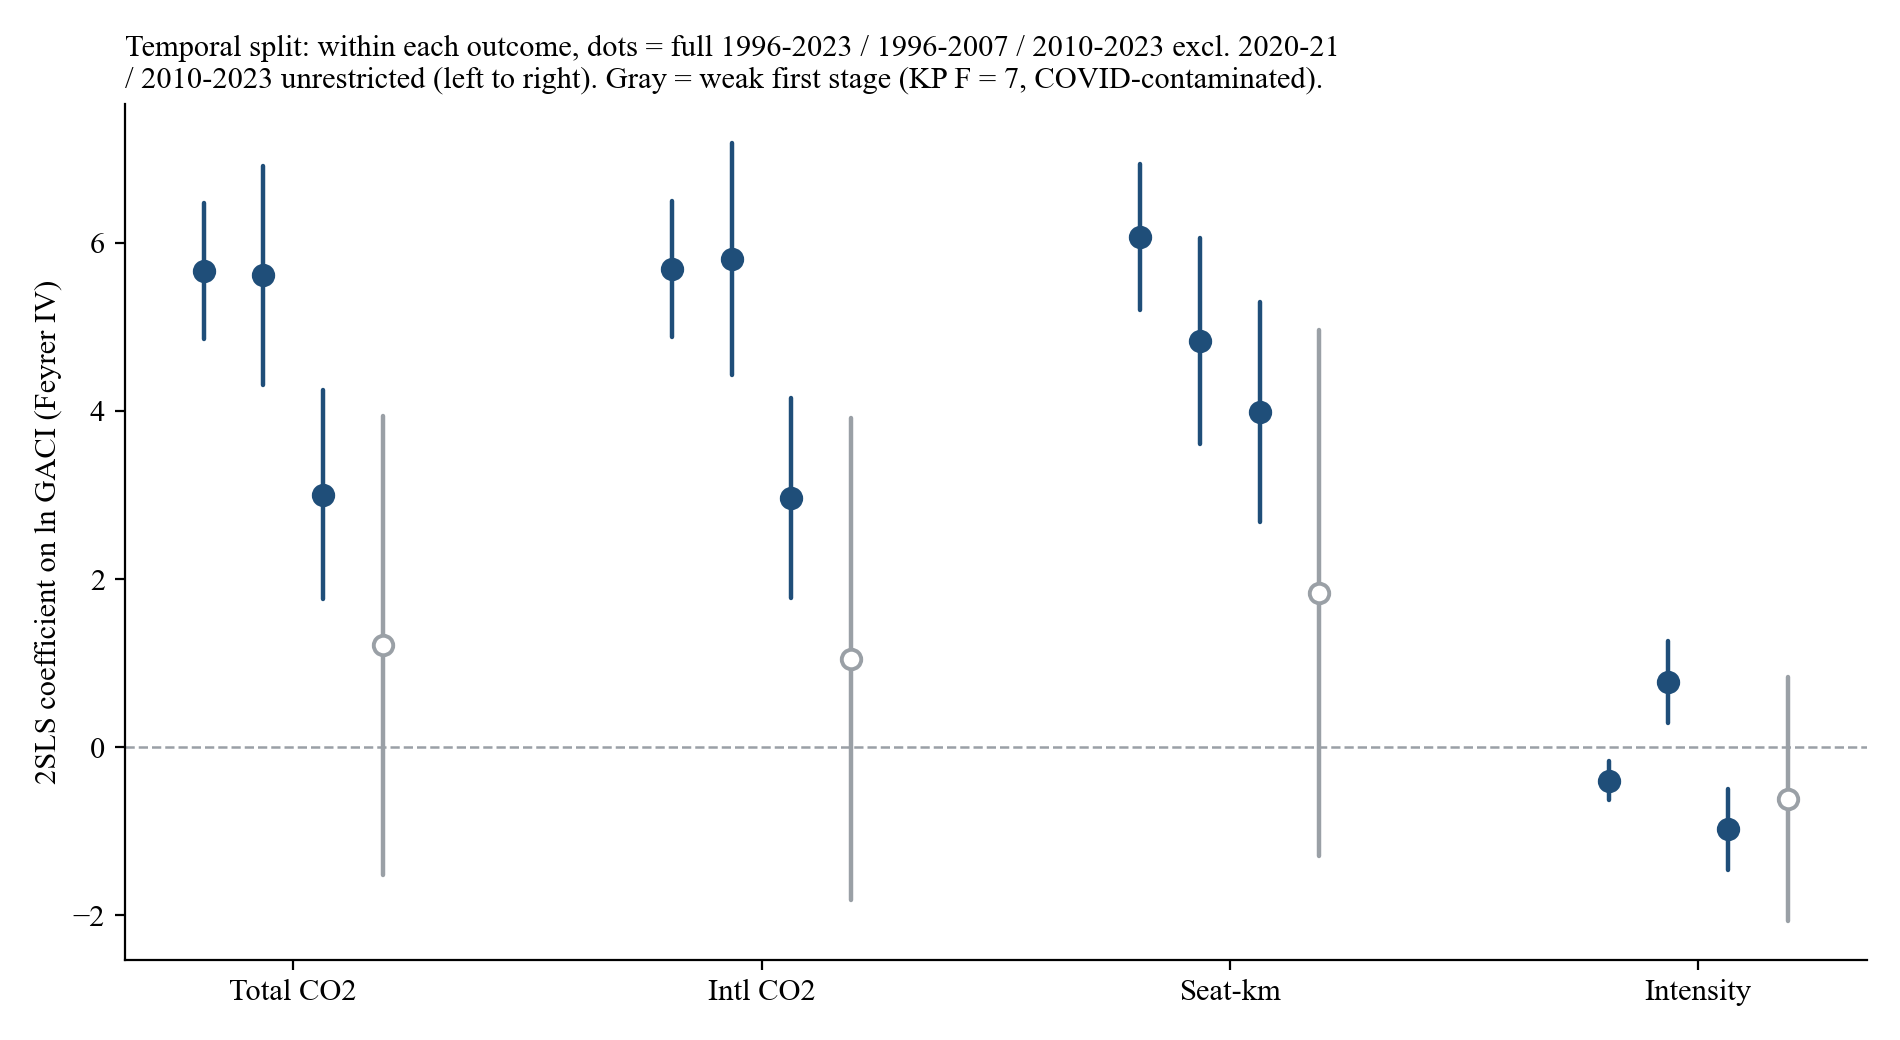
\includegraphics[width=0.92\textwidth]{CO2_temporal_coefplot.png}
\caption{Temporal split of the connectivity elasticity. Within each outcome, markers show the full sample, the network-expansion era (1996--2007), the mature-network era (2010--2023 excluding the COVID-19 years 2020--2021), and the unrestricted 2010--2023 sample from left to right; gray denotes the unrestricted later sample, whose first stage (KP $F=7$) is contaminated by the COVID collapse.}
\label{fig:temporal}
\end{figure}

\subsection{Heterogeneity of the elasticity}
Because the world average combines countries entering the network with
countries already saturated, Table~\ref{tab:hetero} splits the sample by
1996 characteristics. The gradient is monotone and steep. The elasticity is
11.43 in the bottom income tercile, 5.91 in the middle, and an
insignificant 0.35 at the top; by baseline connectivity the pattern is the
same (9.02, 5.64, and 0.45, though the high-connectivity first stage is too
weak for inference). Regionally, the elasticity is 8.39 in Africa, 5.42 in
Asia--Pacific, and 3.23 in Latin America, while Europe is a precisely
estimated zero (0.24, s.e.\ 0.62); the Middle East and North America have
too little instrument variation to be identified. The technique margin
follows the same geography: emissions per seat-km fall significantly only
in the bottom income tercile (Panel D). The headline elasticity is
therefore an average over network entrants. For mature networks,
connectivity growth is approximately carbon-neutral at the margin, whereas
for entrants both the scale burden and the efficiency gains are
concentrated. Figure~\ref{fig:hetero} plots the estimates.

\begin{table}[htbp]
\centering
\begin{threeparttable}
\caption{Heterogeneity of the connectivity elasticity}
\label{tab:hetero}
\footnotesize
\begin{tabular}{lcccc}
\toprule
 & Coefficient & s.e. & KP $F$ & $N$ \\
\midrule
\multicolumn{5}{l}{\textit{Panel A. Total CO$_2$ by baseline income tercile}} \\
  Low income & 11.431$^{***}$ & (1.338) & 35.2 & 1,595 \\
  Middle income & 5.906$^{***}$ & (0.782) & 48.2 & 1,547 \\
  High income & 0.350 & (1.106) & 10.1 & 1,491 \\
\midrule
\multicolumn{5}{l}{\textit{Panel B. Total CO$_2$ by baseline connectivity tercile}} \\
  Low connectivity & 9.018$^{***}$ & (0.656) & 117.4 & 1,452 \\
  Middle connectivity & 5.642$^{***}$ & (0.908) & 29.9 & 1,526 \\
  High connectivity & 0.452 & (2.201) & 1.8 & 1,655 \\
\midrule
\multicolumn{5}{l}{\textit{Panel C. Total CO$_2$ by region}} \\
  Europe & 0.236 & (0.616) & 55.5 & 1,189 \\
  Asia--Pacific & 5.424$^{***}$ & (0.667) & 64.4 & 1,110 \\
  Africa & 8.385$^{***}$ & (1.688) & 20.2 & 1,230 \\
  Latin America & 3.229$^{***}$ & (0.900) & 14.1 & 683 \\
  Middle East & \multicolumn{4}{c}{not identified (KP $F<2$)} \\
  North America & \multicolumn{4}{c}{not identified (KP $F<2$)} \\
\midrule
\multicolumn{5}{l}{\textit{Panel D. Intensity by baseline income tercile}} \\
  Low income & -1.057$^{***}$ & (0.299) & 35.5 & 1,596 \\
  Middle income & -0.372 & (0.241) & 48.2 & 1,547 \\
  High income & 1.012 & (0.715) & 10.1 & 1,491 \\
\bottomrule
\end{tabular}
\begin{tablenotes}[flushleft]
\footnotesize
\item Notes: Split-sample 2SLS with the Feyrer instrument; terciles are formed on 1996 values. All specifications include country and year fixed effects and control for log population and log sea market access. The Middle East and North America cells have too little instrument variation for inference. Robust standard errors in parentheses. $^{***}$, $^{**}$, $^{*}$: significance at 1, 5, and 10 percent.
\end{tablenotes}
\end{threeparttable}
\end{table}

\begin{figure}[htbp]
\centering
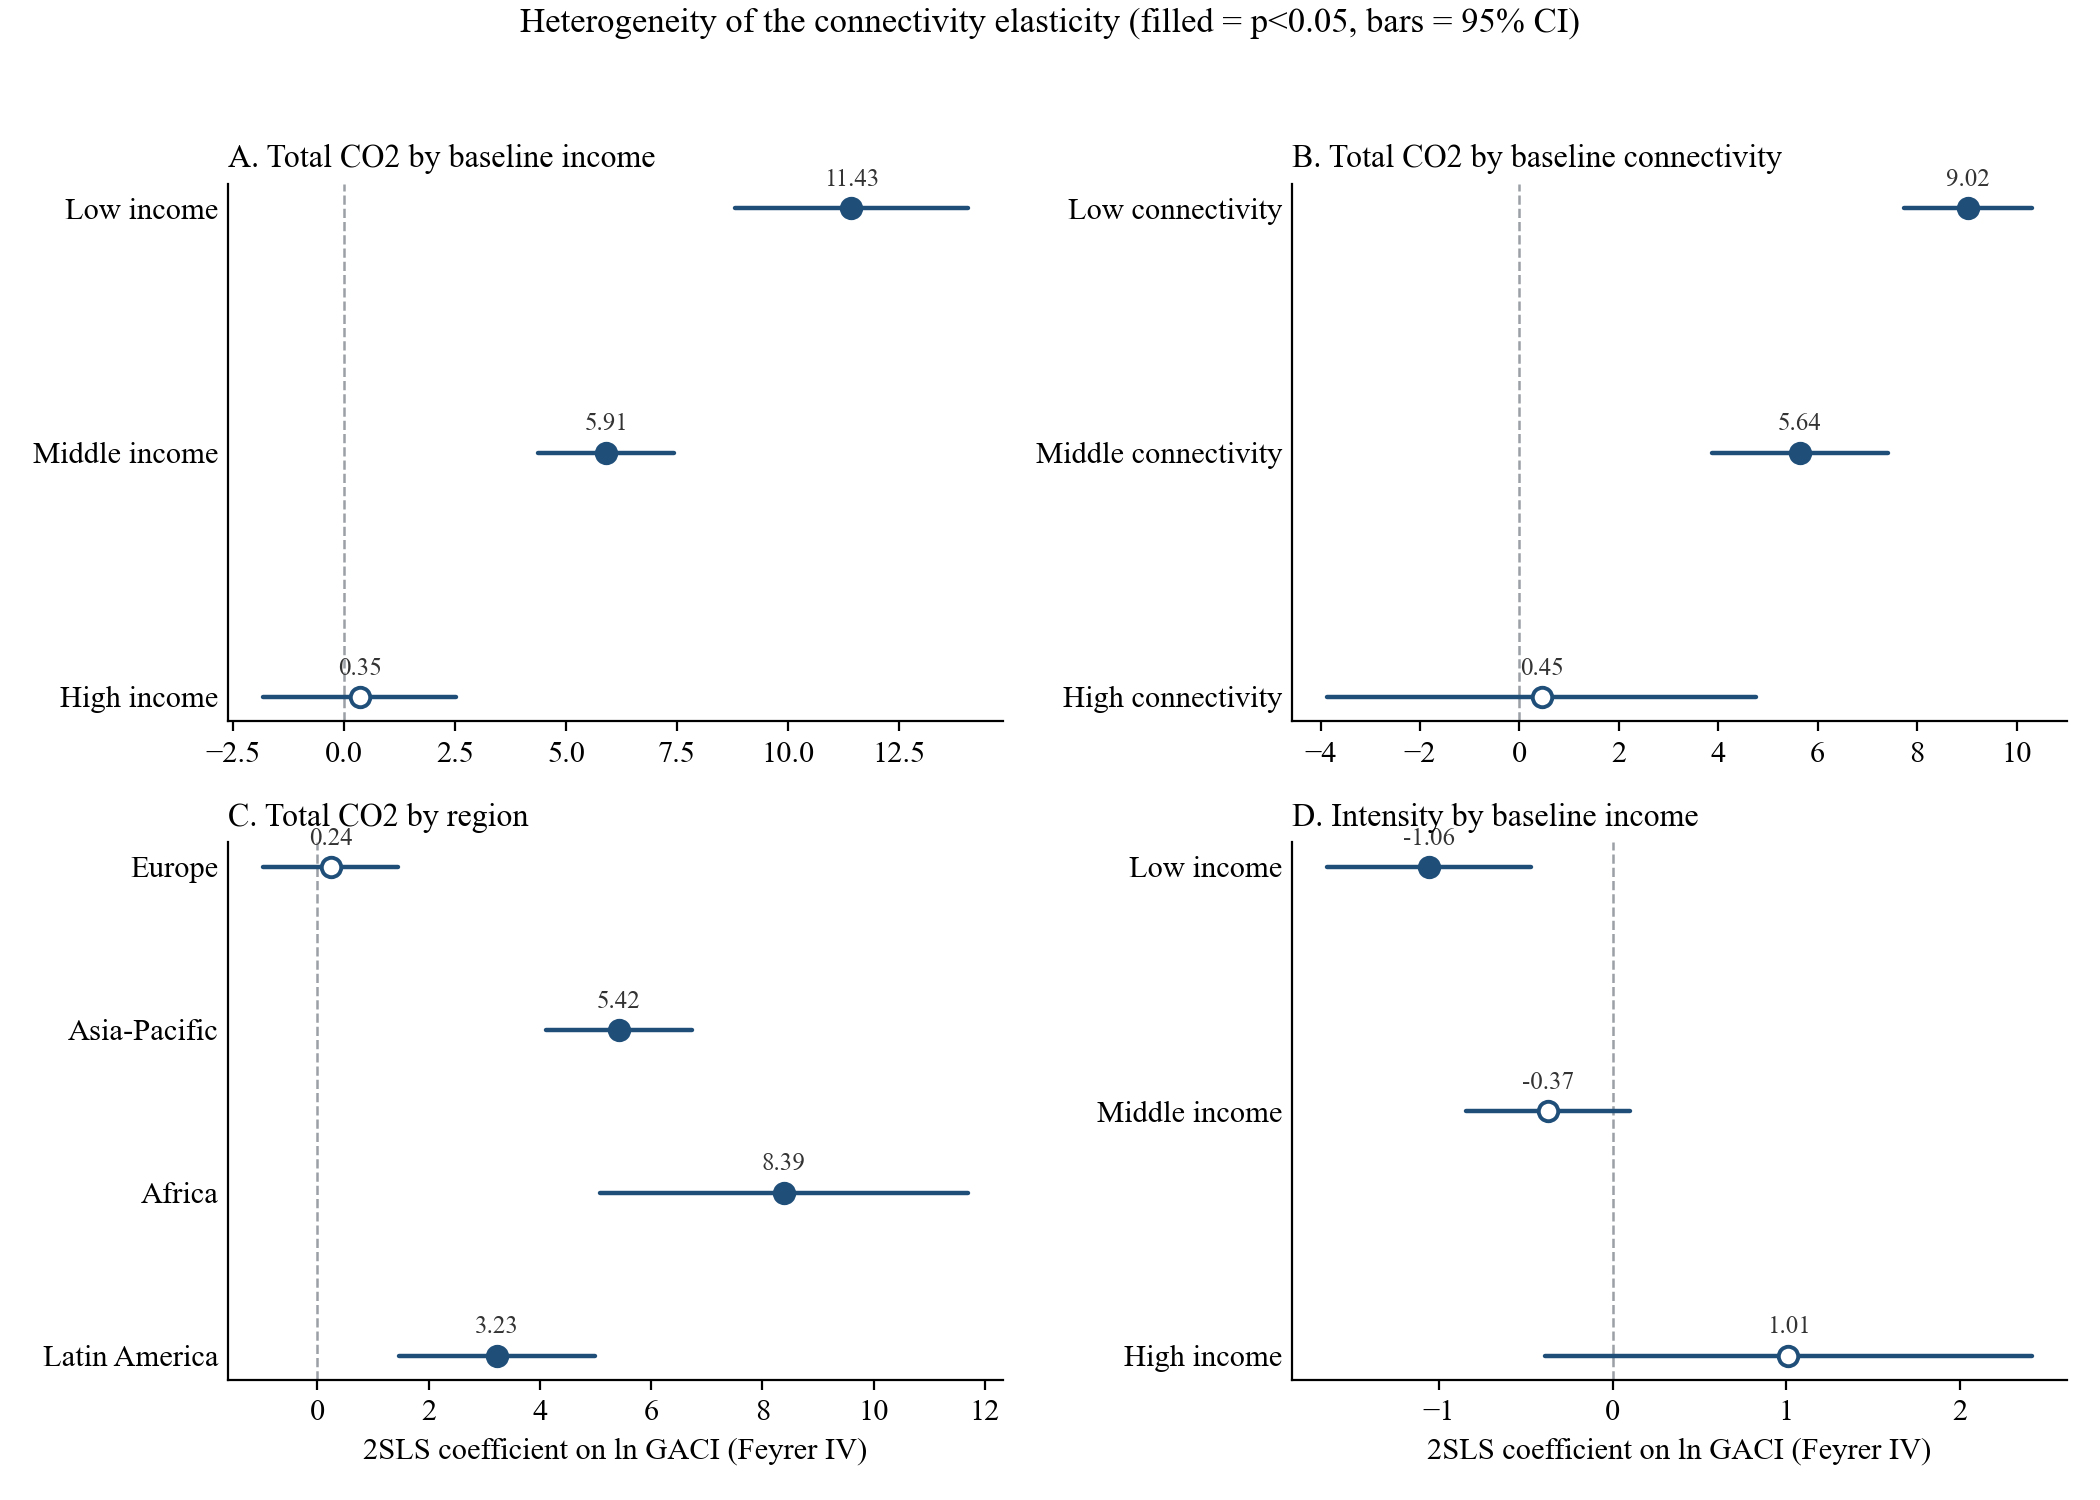
\includegraphics[width=0.92\textwidth]{CO2_hetero_coefplot.png}
\caption{Heterogeneity of the connectivity elasticity (2SLS, Feyrer instrument). Filled markers denote $p<0.05$; bars are 95 percent confidence intervals. The Middle East and North America are omitted as unidentified.}
\label{fig:hetero}
\end{figure}

\subsection{Mechanisms}
Table~\ref{tab:mediation} examines which margin transmits the effect. In
the instrumental-variable product-of-coefficients decomposition,
seat-kilometres mediate 86.5 percent of the total effect (ACME 4.90, Sobel
$p<0.001$) and flight frequency 83.9 percent, while the international share
mediates essentially nothing ($-1.8$ percent). The Imai, Keele and Yamamoto
estimates on the OLS scale agree, attributing 95.6 percent to
seat-kilometres. The connectivity-emissions relationship is thus a
traffic-volume phenomenon, transmitted through additional service rather
than through a recomposition of the network toward international flying.
Composition does respond to connectivity, but through a different kind of
variation, examined next.

\begin{table}[htbp]
\centering
\begin{threeparttable}
\caption{Causal mediation of the connectivity effect on aviation CO$_2$}
\label{tab:mediation}
\footnotesize
\begin{tabular}{lccccc}
\toprule
\multicolumn{6}{l}{\textit{Panel A. Instrumental-variable product of coefficients (2SLS scale; total effect 5.669)}} \\
Mediator & $a$: GACI$\rightarrow M$ & $b$: $M\rightarrow$CO$_2$ & ACME ($a\times b$) & Sobel $p$ & Share mediated \\
\midrule
  Flight frequency & 6.976 & 0.682 & 4.756 & 0.000 & 83.9\% \\
  Seat-kilometres & 6.068 & 0.808 & 4.901 & 0.000 & 86.5\% \\
  International share & 0.096 & -1.060 & -0.102 & 0.060 & -1.8\% \\
\midrule
\multicolumn{6}{l}{\textit{Panel B. Imai, Keele and Yamamoto (2010) mediation (OLS scale; total effect 3.582)}} \\
Mediator & ACME & Direct effect & Total effect & & Share mediated \\
\midrule
  Flight frequency & 1.766 & 1.816 & 3.582 & & 49.3\% \\
  Seat-kilometres & 3.424 & 0.159 & 3.583 & & 95.6\% \\
  International share & -0.077 & 3.657 & 3.580 & & -2.1\% \\
\bottomrule
\end{tabular}
\begin{tablenotes}[flushleft]
\footnotesize
\item Notes: Outcome is log total bunker CO$_2$; the treatment is log GACI (capacity-weighted mean). Panel A instruments the treatment with the Feyrer shifter in each equation and combines the paths by the product method with delta-method (Sobel) standard errors. Panel B implements the algorithm of Imai, Keele and Yamamoto (2010) by quasi-Bayesian simulation (200 draws) on least-squares models with country and year indicator variables. Each row is a separate single-mediator analysis and the mediators overlap, so shares do not sum across rows. All models control for log population and log sea market access. Sequential ignorability of the mediator is assumed conditional on the fixed effects.
\end{tablenotes}
\end{threeparttable}
\end{table}

\subsection{The composition margin: evidence from the tourism instrument}
The tourism-heritage instrument identifies from hub-quality changes rather
than from geographic market access, and it yields a complementary result.
Under this instrument, total emissions do not respond (1.16, s.e.\ 0.86),
but international emissions rise by 3.16 percent (s.e.\ 0.77) and emissions
per seat-km by 1.23 percent (s.e.\ 0.46): hub-quality gains recompose
traffic toward international long-haul service rather than scaling it. We
present this as evidence on the composition margin while disclosing that
the instrument does not survive the size-by-cycle stress test (Appendix A).
The two instruments have different complier populations, and their
divergence is informative about which margin each kind of connectivity
variation moves.

\subsection{Connectivity spillovers}
Emissions do not respond only to a country's own network.
Table~\ref{tab:spillover} instruments the inverse-distance-weighted
connectivity of all other countries with their Feyrer shifters, holding the
own shifter fixed. The spillover is large: a one percent increase in
neighbours' connectivity raises own bunker CO$_2$ by 7.45 percent (s.e.\
1.99) and international CO$_2$ by 10.24 percent, and raises emissions per
seat-km (1.31, s.e.\ 0.53). Trade volume does not respond (2.07, s.e.\
2.01), so the channel is a change in the structure of aviation activity
rather than trade demand. Panel B identifies the margins: flight frequency
does not move, but seat-kilometres rise by 6.14 percent through larger
aircraft (5.44) and a more international traffic mix (1.05), with shorter
stage lengths ($-2.03$). This pattern is the converse of the own-connectivity
response, which operates through frequency: when neighbouring hubs grow, a
country's own traffic shifts toward larger-gauge, more international
service, consistent with feeding traffic into foreign hubs. Two
implications follow. First, single-country estimates understate the
network-wide emissions effect of connectivity growth. Second, the emissions
accrue across borders while the associated economic gains, as proxied by
trade, show no measurable response, which sharpens the attribution
questions taken up in Section 6.

\begin{table}[htbp]
\centering
\begin{threeparttable}
\caption{Connectivity spillovers: neighbouring countries' connectivity and own aviation outcomes}
\label{tab:spillover}
\footnotesize
\begin{tabular}{lccccc}
\toprule
\multicolumn{6}{l}{\textit{Panel A. 2SLS: neighbour connectivity instrumented}} \\
 & \multicolumn{1}{c}{Bunker CO$_2$} & \multicolumn{1}{c}{Intl.\ CO$_2$} & \multicolumn{1}{c}{Intensity} & \multicolumn{1}{c}{Trade volume} & \\
 & (1) & (2) & (3) & (4) & \\
\midrule
  ln neighbour GACI & 7.454$^{***}$ & 10.237$^{***}$ & 1.312$^{**}$ & 2.072 & \\
   & (1.994) & (2.092) & (0.534) & (2.011) & \\
  Own Feyrer shifter & 0.254$^{**}$ & 0.076 & -0.134$^{***}$ & 0.157 & \\
   & (0.122) & (0.128) & (0.037) & (0.124) & \\
  KP $F$ & 134.1 & 134.0 & 134.1 & 134.1 & \\
  $N$ & 4,623 & 4,622 & 4,623 & 4,623 & \\
\midrule
\multicolumn{6}{l}{\textit{Panel B. Margins of the own response to neighbour connectivity (same specification)}} \\
 & \multicolumn{1}{c}{Flights} & \multicolumn{1}{c}{Seat-km} & \multicolumn{1}{c}{Aircraft size} & \multicolumn{1}{c}{Stage length} & \multicolumn{1}{c}{Intl.\ share} \\
 & (1) & (2) & (3) & (4) & (5) \\
\midrule
  ln neighbour GACI & 2.730 & 6.141$^{***}$ & 5.437$^{***}$ & -2.026$^{**}$ & 1.046$^{***}$ \\
   & (2.216) & (2.083) & (1.170) & (1.008) & (0.281) \\
\bottomrule
\end{tabular}
\begin{tablenotes}[flushleft]
\footnotesize
\item Notes: Neighbour connectivity is the inverse-distance-weighted average of all other countries' log GACI (capacity-weighted mean), with weights based on haversine distances between countries' aviation activity centroids. It is instrumented by the identically weighted average of other countries' Feyrer shifters; the own Feyrer shifter enters directly, so the own-connectivity effect is in reduced form. Own and neighbour connectivity cannot be jointly instrumented because the two shifters are collinear within country. All specifications include country and year fixed effects and control for log population and log sea market access. Robust standard errors in parentheses. $^{***}$, $^{**}$, $^{*}$: significance at 1, 5, and 10 percent.
\end{tablenotes}
\end{threeparttable}
\end{table}

\subsection{Airport-level evidence on the technique margin}
The country-level intensity decline has a within-country counterpart. In an
airport panel with airport and country-by-year fixed effects, a one percent
increase in an airport's connectivity is associated with a 0.49 percent
decline in CO$_2$ per seat-km (s.e.\ 0.04) and a 0.33 percentage point
higher international share of seat-kilometres.
Figure~\ref{fig:effcurve} shows the cross-section: median intensity falls
monotonically from 284 to 77 kg per 1{,}000 seat-km across connectivity
ventiles, while the international share rises from one to sixty percent.
These estimates are descriptive, since no valid airport-level instrument is
available (Appendix A), but they locate the technique margin at the node:
airports with higher connectivity operate at substantially lower emissions
per seat-km even as they concentrate long-haul volume.

\begin{figure}[htbp]
\centering
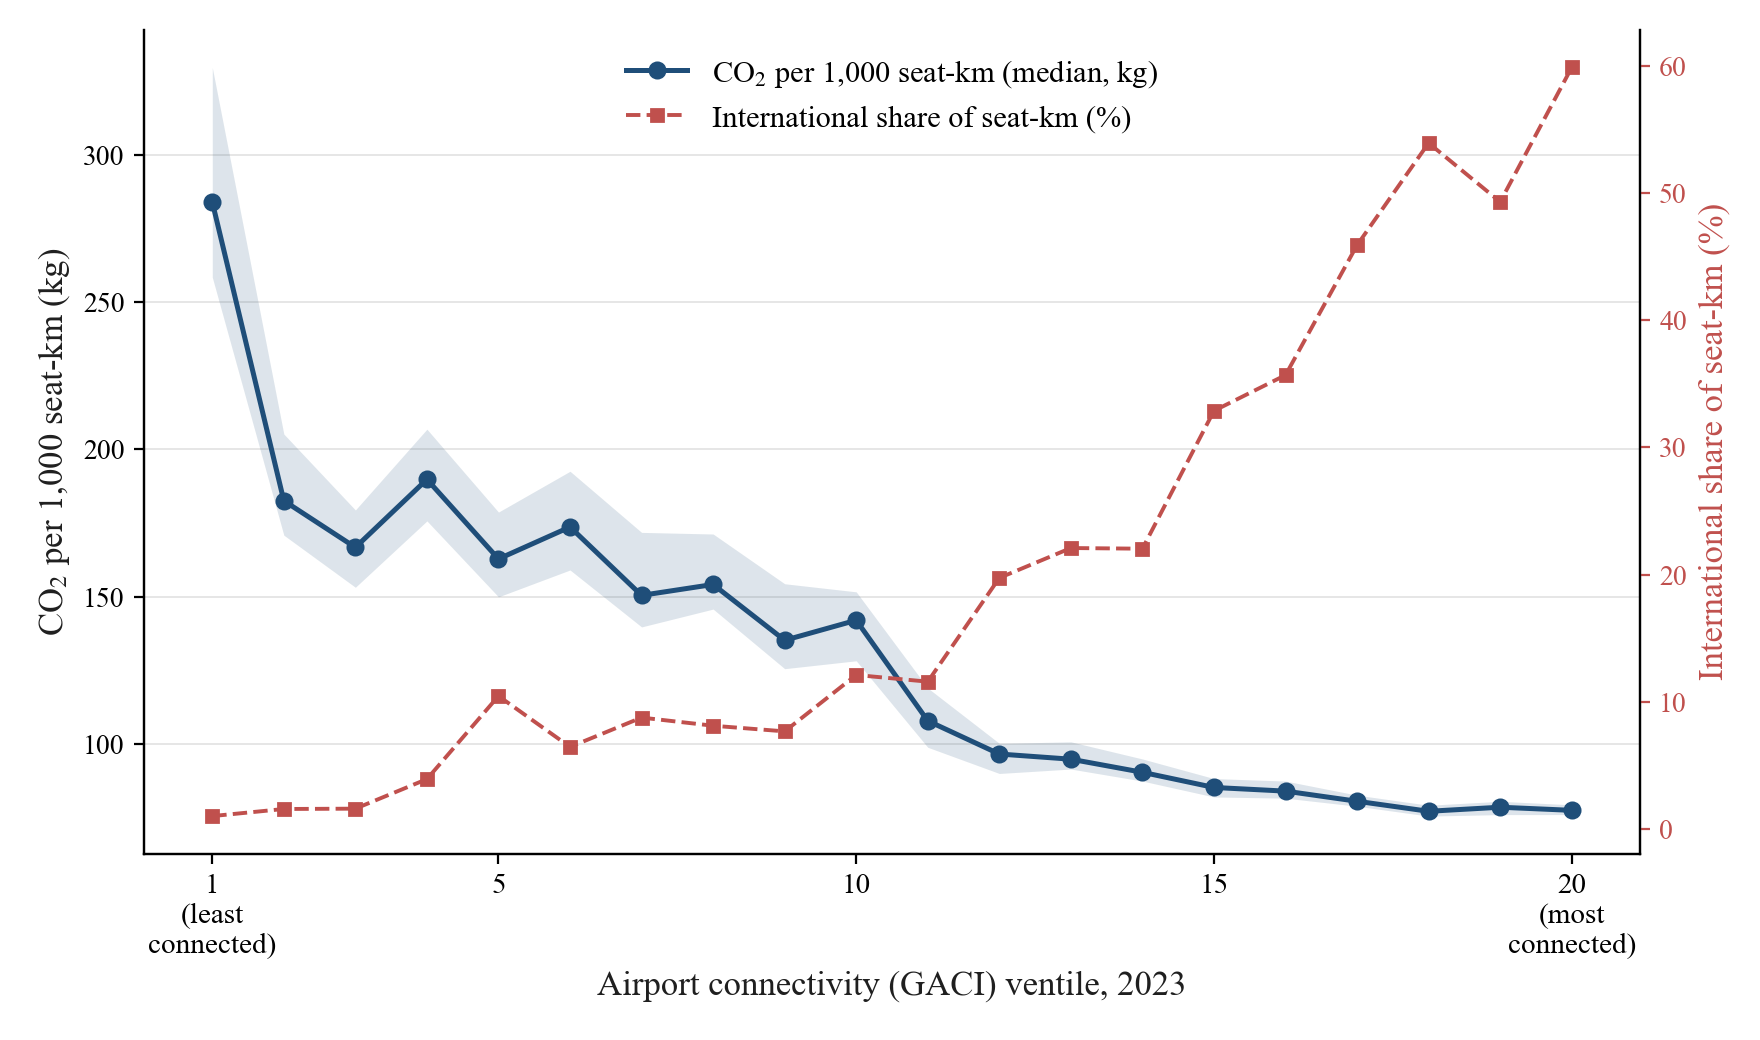
\includegraphics[width=0.92\textwidth]{CO2_efficiency_curve.png}
\caption{Airport-level efficiency curve, 2023: median kg CO$_2$ per 1{,}000 seat-km by connectivity ventile, with the international share of seat-km on the second panel.}
\label{fig:effcurve}
\end{figure}

\subsection{Attribution of 2023 emissions to connectivity growth}
Applying the estimated elasticity to each country's connectivity change
since 1996 attributes 356 Mt, or 42.5 percent, of 2023 aviation CO$_2$ to
post-1996 network expansion (212 Mt and 41.2 percent of international
emissions). The attributed growth is concentrated where networks expanded:
China ($+88$ Mt), the United States ($+36$), the United Arab Emirates
($+25$), Japan ($+17$), Turkey ($+17$), India ($+16$), and Korea ($+14$),
while Germany's declining connectivity contributes $-16$ Mt.
Figures~\ref{fig:dlngaci} and \ref{fig:attributed} map the connectivity
change and the attributed emissions. Because the elasticity is far above
one, country-level attributed shares are extreme for fast-growing
countries; these figures are partial-equilibrium accounting, and the world
total of 42.5 percent is the more conservative summary.

Table~\ref{tab:scc} reports the country-level estimates together with their
monetised social cost. Valued at standard social-cost-of-carbon estimates,
the 356 Mt of 2023 emissions attributable to connectivity growth represent
an annual external cost of \$18.2 billion at the United States Interagency
Working Group interim value (\$51 per tonne), \$65.9 billion at the Rennert
et al.\ estimate (\$185), and \$67.7 billion at the United States EPA
central value (\$190) [TODO cite]. The cost is concentrated in the same
emerging hub countries as the emissions: at the EPA value, \$16.7 billion
per year for China, \$6.9 billion for the United States, and \$4.7 billion
for the United Arab Emirates, while Germany's connectivity decline
corresponds to an avoided cost of \$3.0 billion per year. These are flow
valuations of a single year's attributable emissions and recur annually for
as long as the connectivity-driven traffic persists.

\begin{table}[htbp]
\centering
\begin{threeparttable}
\caption{Country-level attribution and social cost of connectivity-driven aviation CO$_2$, 2023}
\label{tab:scc}
\footnotesize
\begin{tabular}{lcccccc}
\toprule
 & & \multicolumn{2}{c}{Attributed CO$_2$ (Mt)} & \multicolumn{3}{c}{Social cost (\$bn per year)} \\
\cmidrule(lr){3-4}\cmidrule(lr){5-7}
 & $\Delta \ln$ GACI & Total & International & SCC \$51 & SCC \$185 & SCC \$190 \\
\midrule
China          & 0.33  & 87.7  & 16.9  & 4.5  & 16.2 & 16.7 \\
United States  & 0.04  & 36.4  & 13.6  & 1.9  & 6.7  & 6.9  \\
United Arab Emirates & 0.57 & 24.7 & 24.7 & 1.3 & 4.6 & 4.7 \\
Japan          & 0.19  & 17.4  & 10.4  & 0.9  & 3.2  & 3.3  \\
Turkey         & 0.55  & 16.6  & 13.5  & 0.8  & 3.1  & 3.2  \\
India          & 0.19  & 15.9  & 7.6   & 0.8  & 2.9  & 3.0  \\
Korea          & 0.71  & 14.1  & 12.8  & 0.7  & 2.6  & 2.7  \\
Canada         & 0.22  & 13.1  & 8.5   & 0.7  & 2.4  & 2.5  \\
Qatar          & 0.80  & 12.2  & 12.2  & 0.6  & 2.3  & 2.3  \\
Spain          & 0.14  & 11.8  & 9.5   & 0.6  & 2.2  & 2.3  \\
Germany        & $-0.09$ & $-15.8$ & $-15.2$ & $-0.8$ & $-2.9$ & $-3.0$ \\
\midrule
World          &       & 356.4 & 212.0 & 18.2 & 65.9 & 67.7 \\
\bottomrule
\end{tabular}
\begin{tablenotes}[flushleft]
\footnotesize
\item Notes: Attributed CO$_2$ applies the Feyrer-instrument elasticities (5.669 total, 5.690 international) to each country's 1996--2023 change in log connectivity: attributed share $= 1-\exp(-\beta\,\Delta\ln\mathrm{GACI}_c)$, applied to 2023 emission levels under the bunker convention. Social cost values one year's attributable emissions at three social-cost-of-carbon estimates (2020 USD per tonne of CO$_2$): the US Interagency Working Group interim value (\$51, 3 percent discount rate), Rennert et al.\ (2022) (\$185, 2 percent near-term discount rate), and the US EPA (2023) central value (\$190, 2 percent Ramsey discounting); the valuation recurs annually while the traffic persists. Top ten positive countries, Germany (largest negative), and the world total (184 countries); the world attributed total equals 42.5 percent of 2023 aviation CO$_2$. Because the elasticity exceeds one, country-level attributed shares are extreme for fast growers; the figures are partial-equilibrium accounting.
\end{tablenotes}
\end{threeparttable}
\end{table}

\begin{figure}[htbp]
\centering
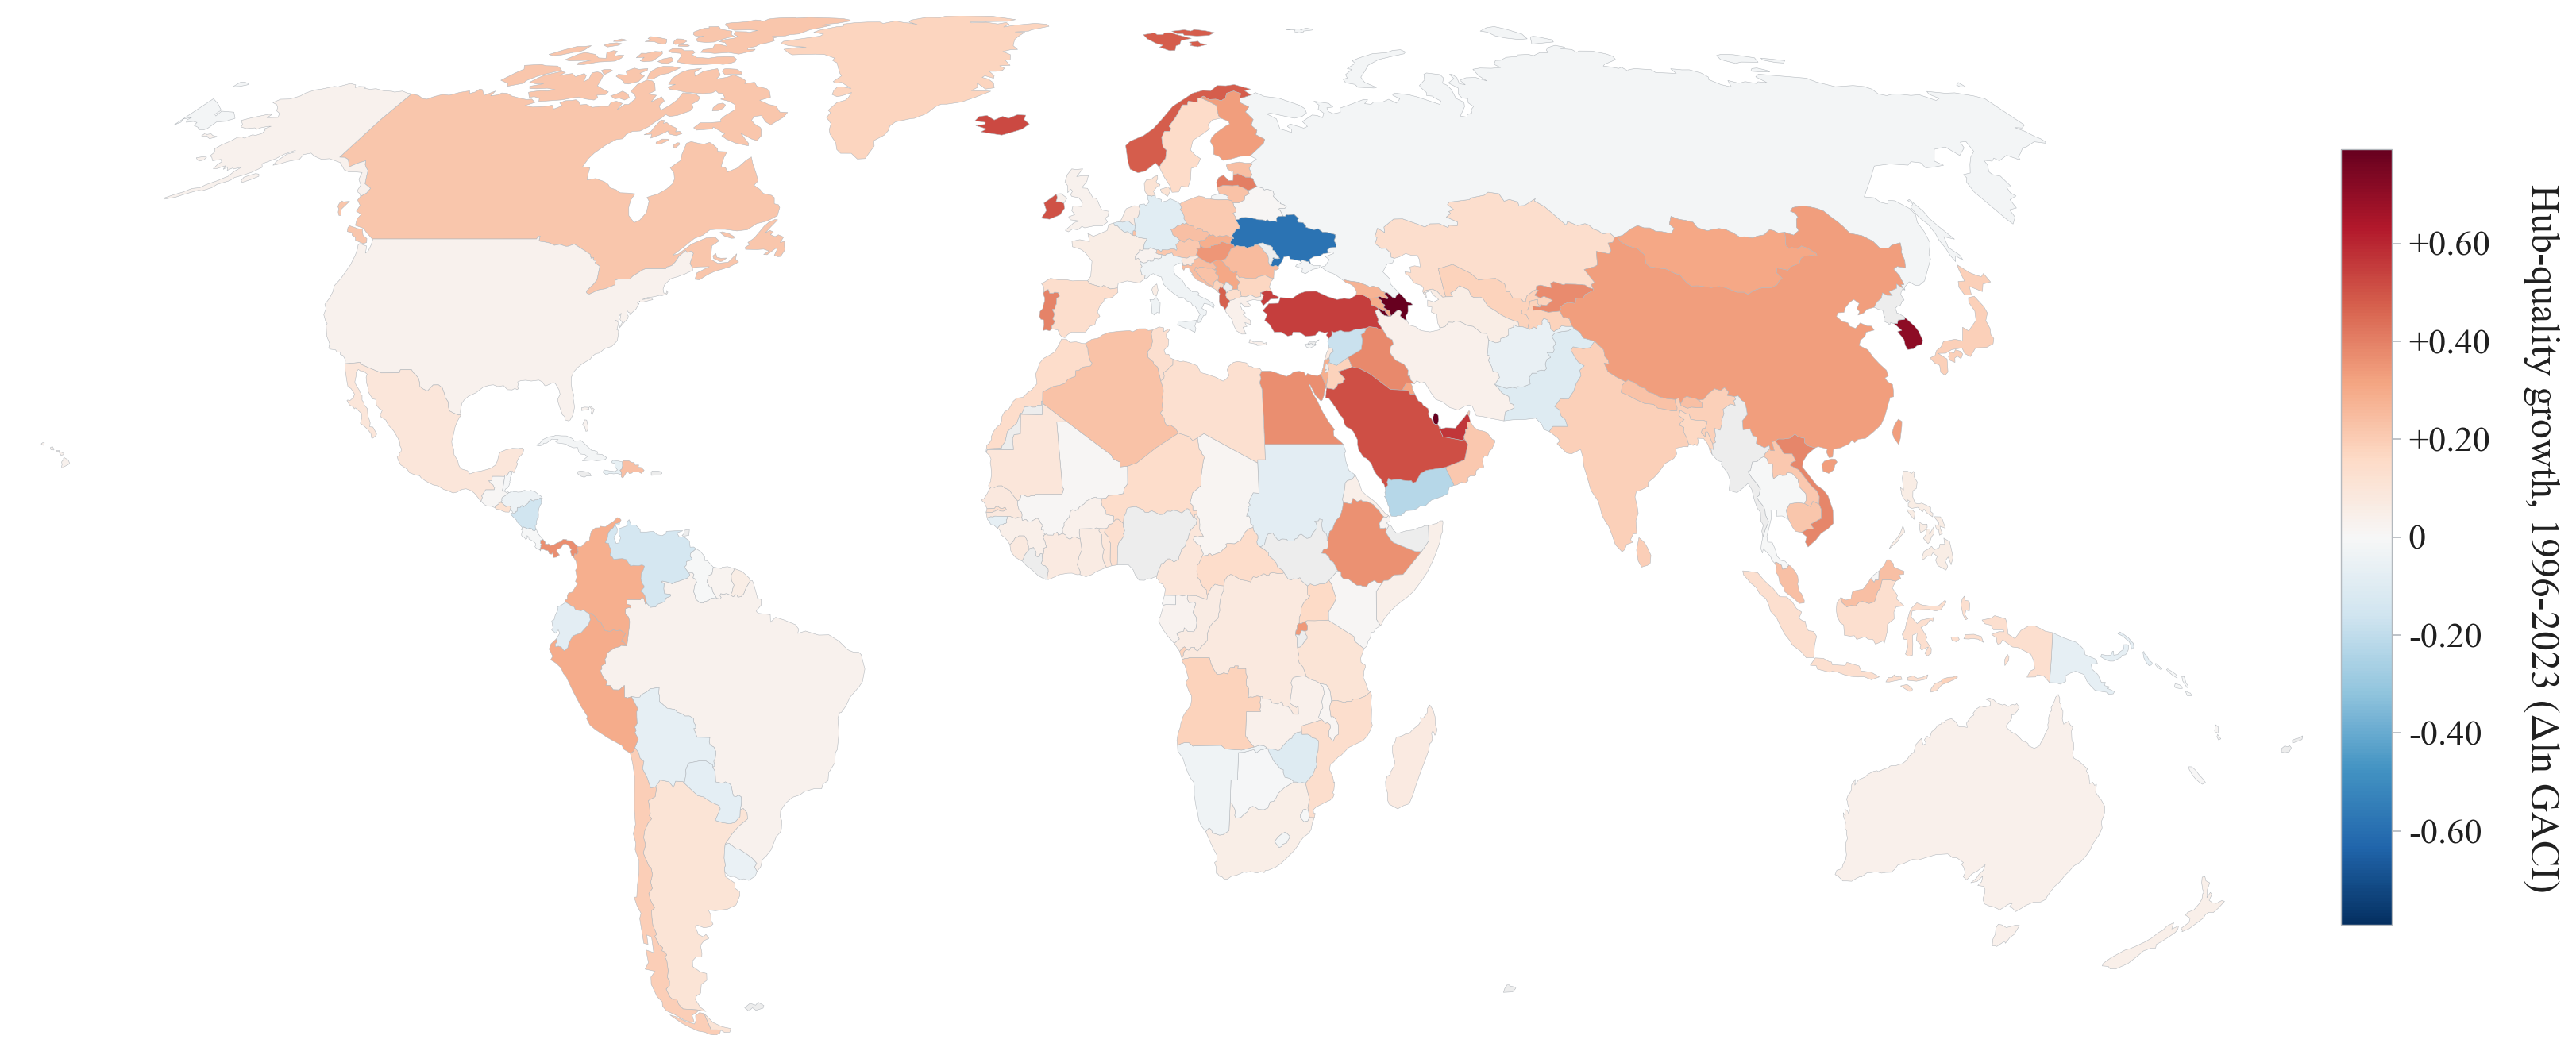
\includegraphics[width=0.92\textwidth]{CO2_map_dlngaci.png}
\caption{Change in log air connectivity (GACI, capacity-weighted mean), 1996--2023.}
\label{fig:dlngaci}
\end{figure}

\begin{figure}[htbp]
\centering
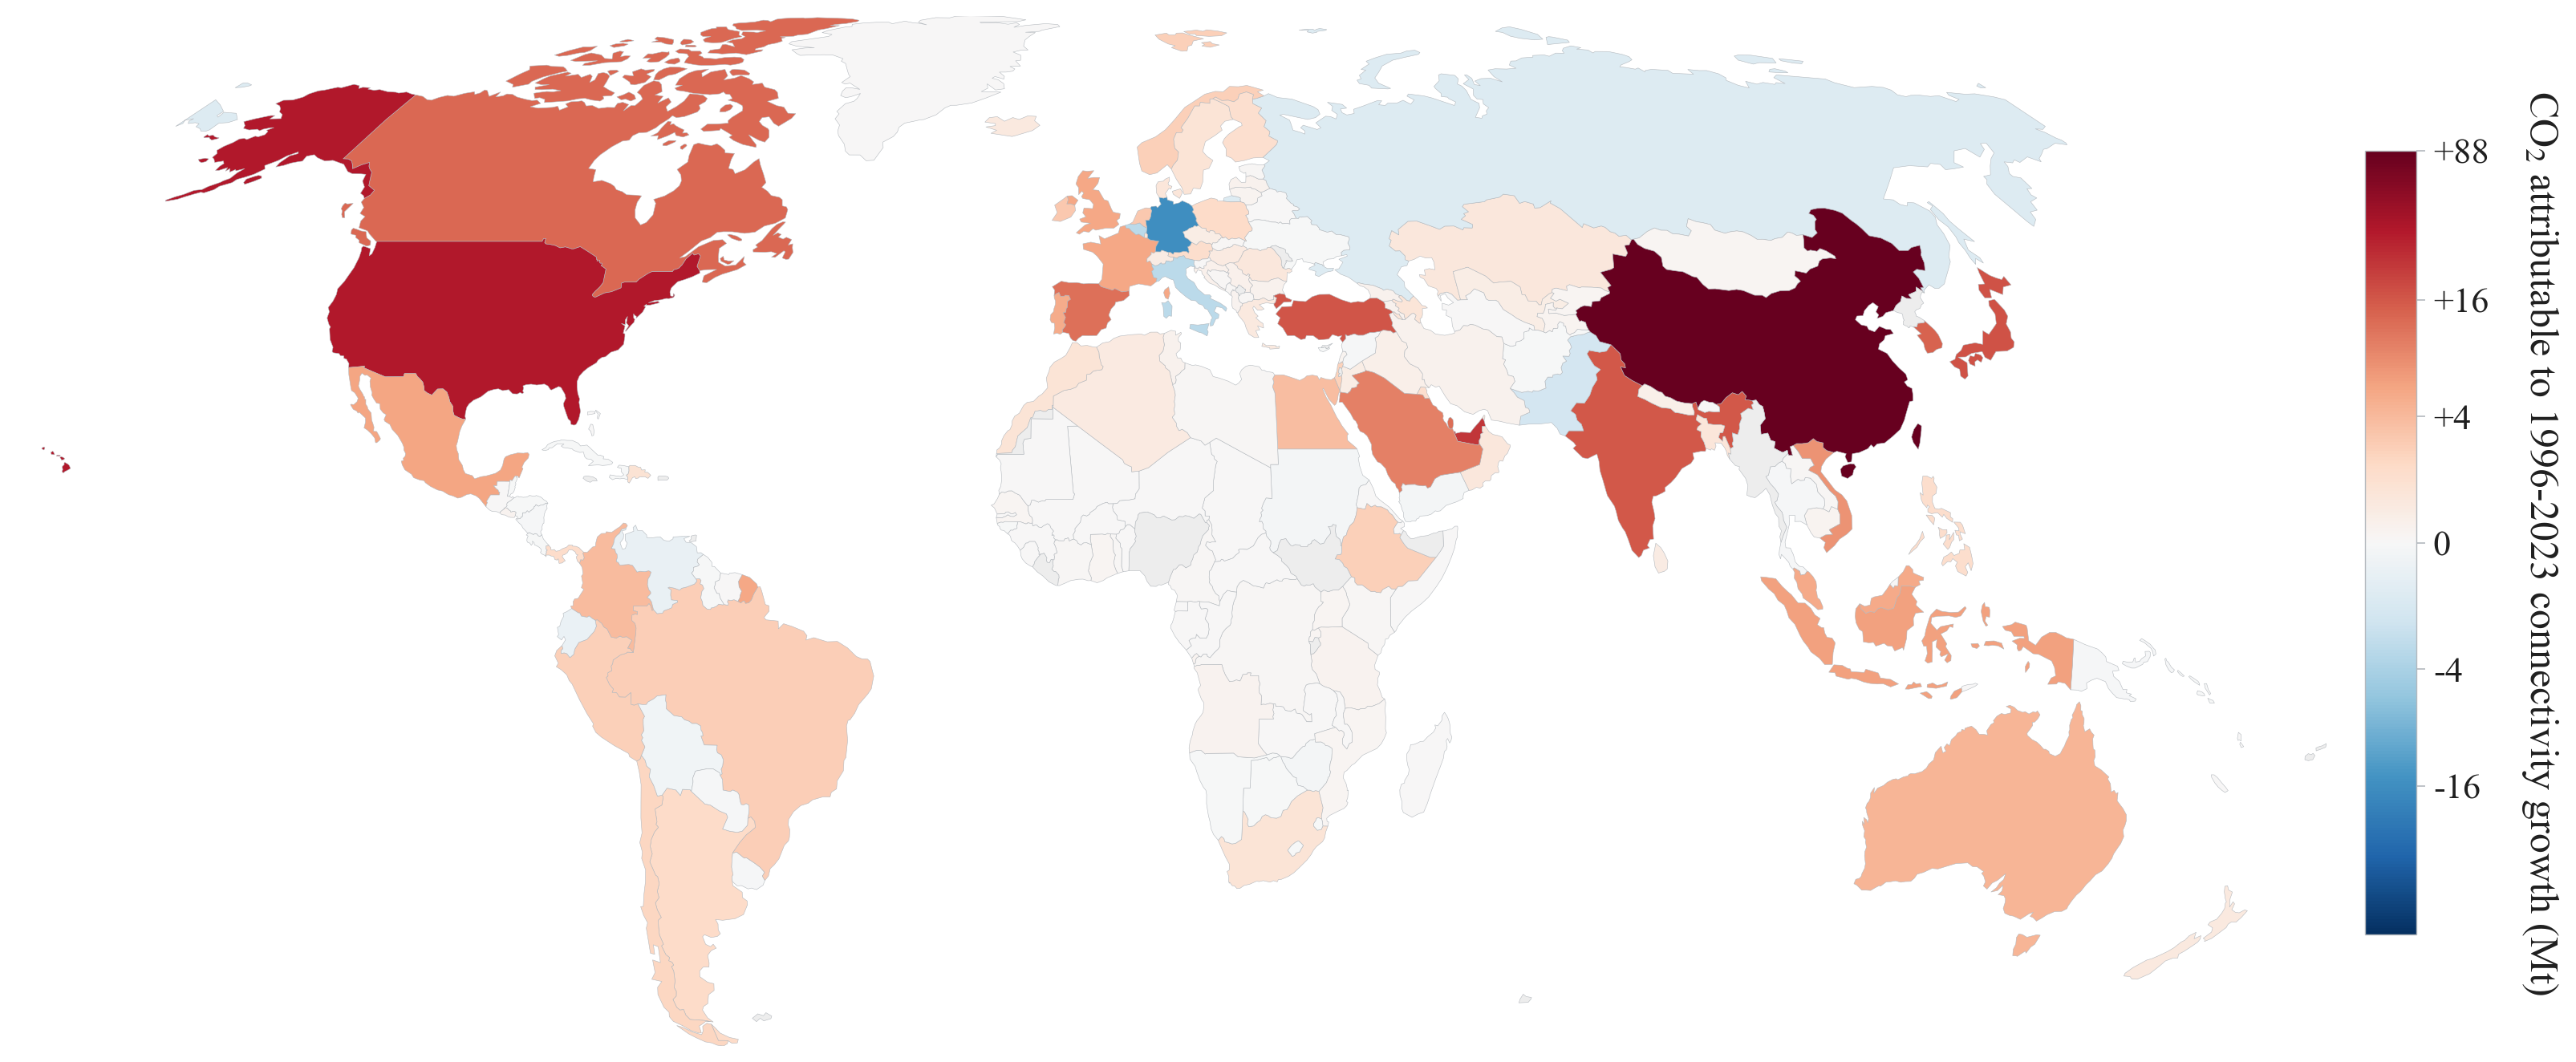
\includegraphics[width=0.92\textwidth]{CO2_map_attributed_2023.png}
\caption{Aviation CO$_2$ attributed to post-1996 connectivity growth, 2023 (Mt). White denotes zero; the attribution applies the Feyrer-instrument elasticity to each country's connectivity change.}
\label{fig:attributed}
\end{figure}

\subsection{Sustainable aviation fuel scenarios}
Since the efficiency margin improves with connectivity but does not offset
the scale margin, the level of emissions can be materially lowered only by
changing the fuel burned. Backing fuel quantities out of the 2023 total of
838 Mt and applying ReFuelEU-style blending paths, the 2035 mandate lowers
the total to 704--754 Mt and the 2050 mandate to 369--545 Mt, depending on
whether the life-cycle saving of sustainable aviation fuel is 80, 65, or 50
percent (Figure~\ref{fig:saf}). Read against the attribution estimate, the
full 2050 blending path with a life-cycle saving of at least 65 percent
would offset emissions of the same magnitude as those attributed to the
connectivity growth of the past generation.

\begin{figure}[htbp]
\centering
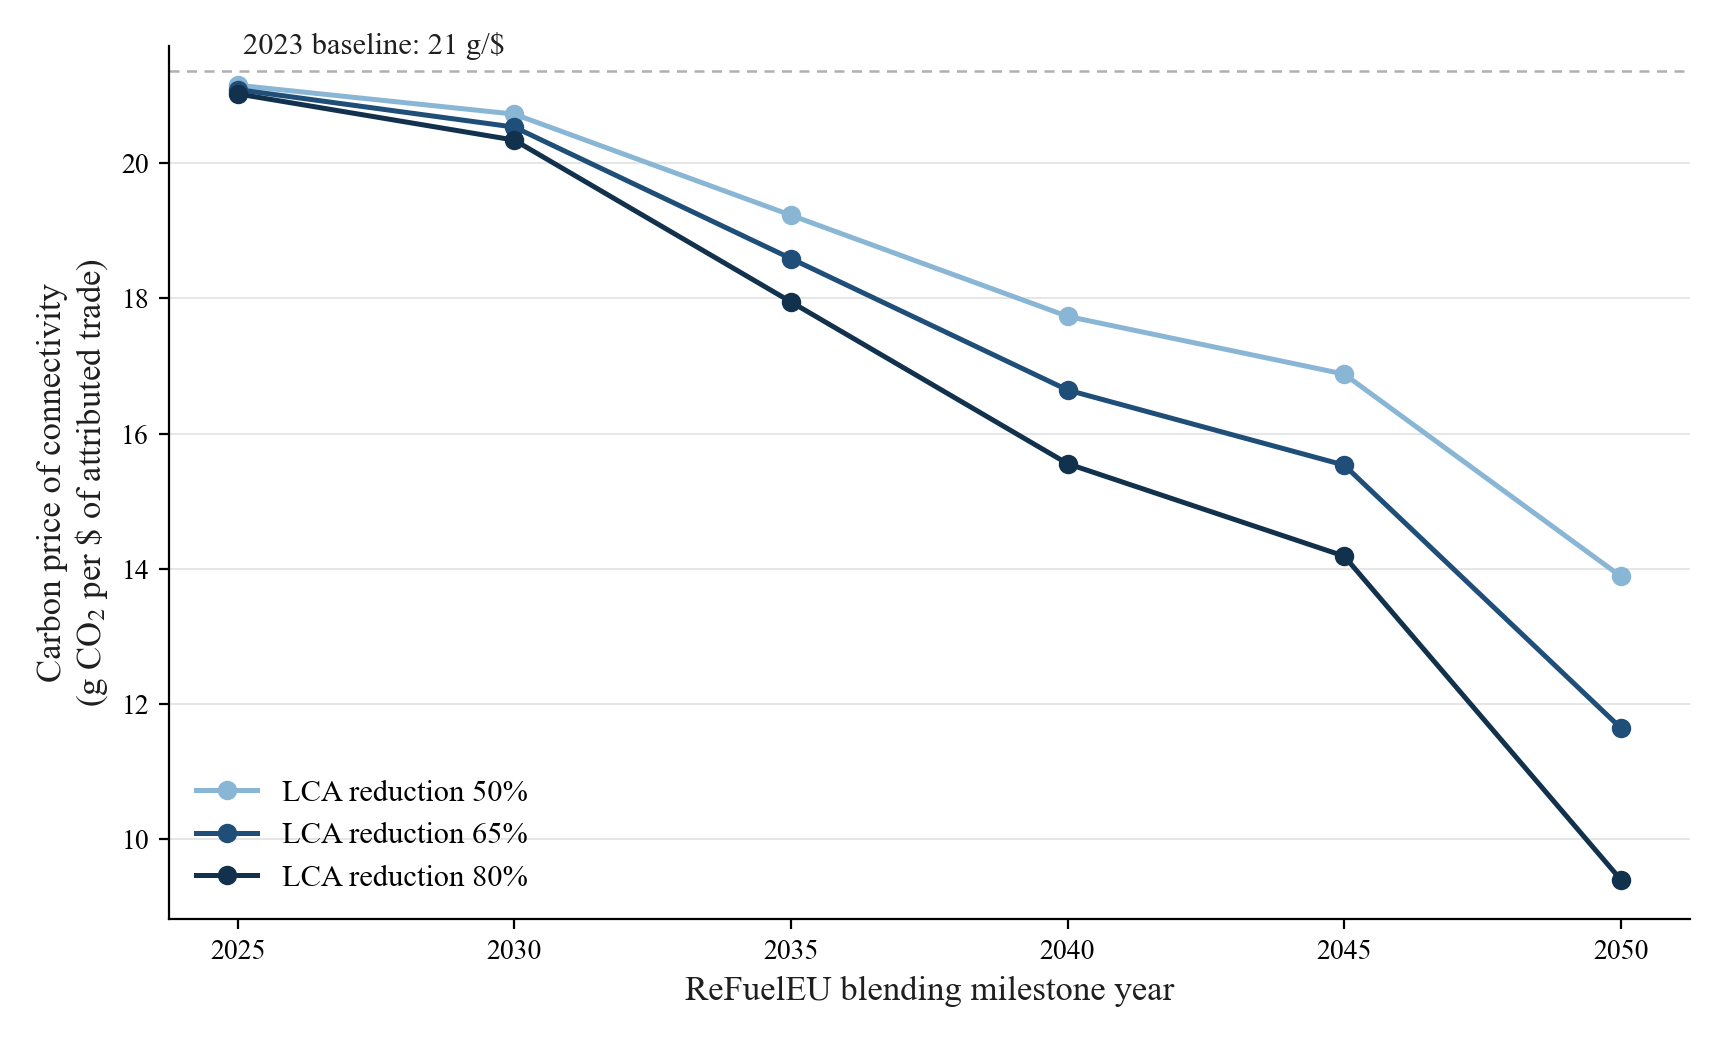
\includegraphics[width=0.92\textwidth]{CO2_saf_scenarios.png}
\caption{World aviation CO$_2$ under ReFuelEU-style SAF blending paths.}
\label{fig:saf}
\end{figure}

%=======================================================================
\section{The geography of attribution}
%=======================================================================
Where connectivity-driven emissions are generated is not where they are
booked. Three descriptive facts organise the maps in
Figures~\ref{fig:levels} and \ref{fig:mismatch}. First, endpoint mismatch
nets out: because scheduled traffic is close to round-trip symmetric,
departure- and arrival-side cruise totals differ by at most 0.7 Mt for any
country, so the binding accounting margin is not which endpoint is assigned
a flight but whether cruise emissions are attributed at all, that is,
bunker attribution versus physical LTO. Second, the mismatch has a clear
geography: the bunker-attributed share of world emissions exceeds the
physical LTO share by 1.4 percentage points for the United States and the
United Arab Emirates, 1.0 for the United Kingdom, and 0.7 for Qatar and
Singapore, while China's attributed share falls short by 3.5 points, with
Japan, Indonesia, and India each around $-0.5$. The airport decomposition
shows the source of the pattern: the gap is positive at every international
mega-hub (LHR $+1.17$, DXB $+1.11$) and negative at large domestically
oriented hubs. Third, combining these facts with the attribution estimates
of Section 5.8, the countries where connectivity growth generated emissions,
notably emerging hub countries, are not the countries where those emissions
are booked under fuel-uplift accounting. Any scheme that allocates
responsibility by booked emissions, including CORSIA, therefore embeds a
transfer across these accounting boundaries. [FANGYU: base-year bilateral
route shares would allow the mismatch to be traced along network links.]

\begin{figure}[htbp]
\centering
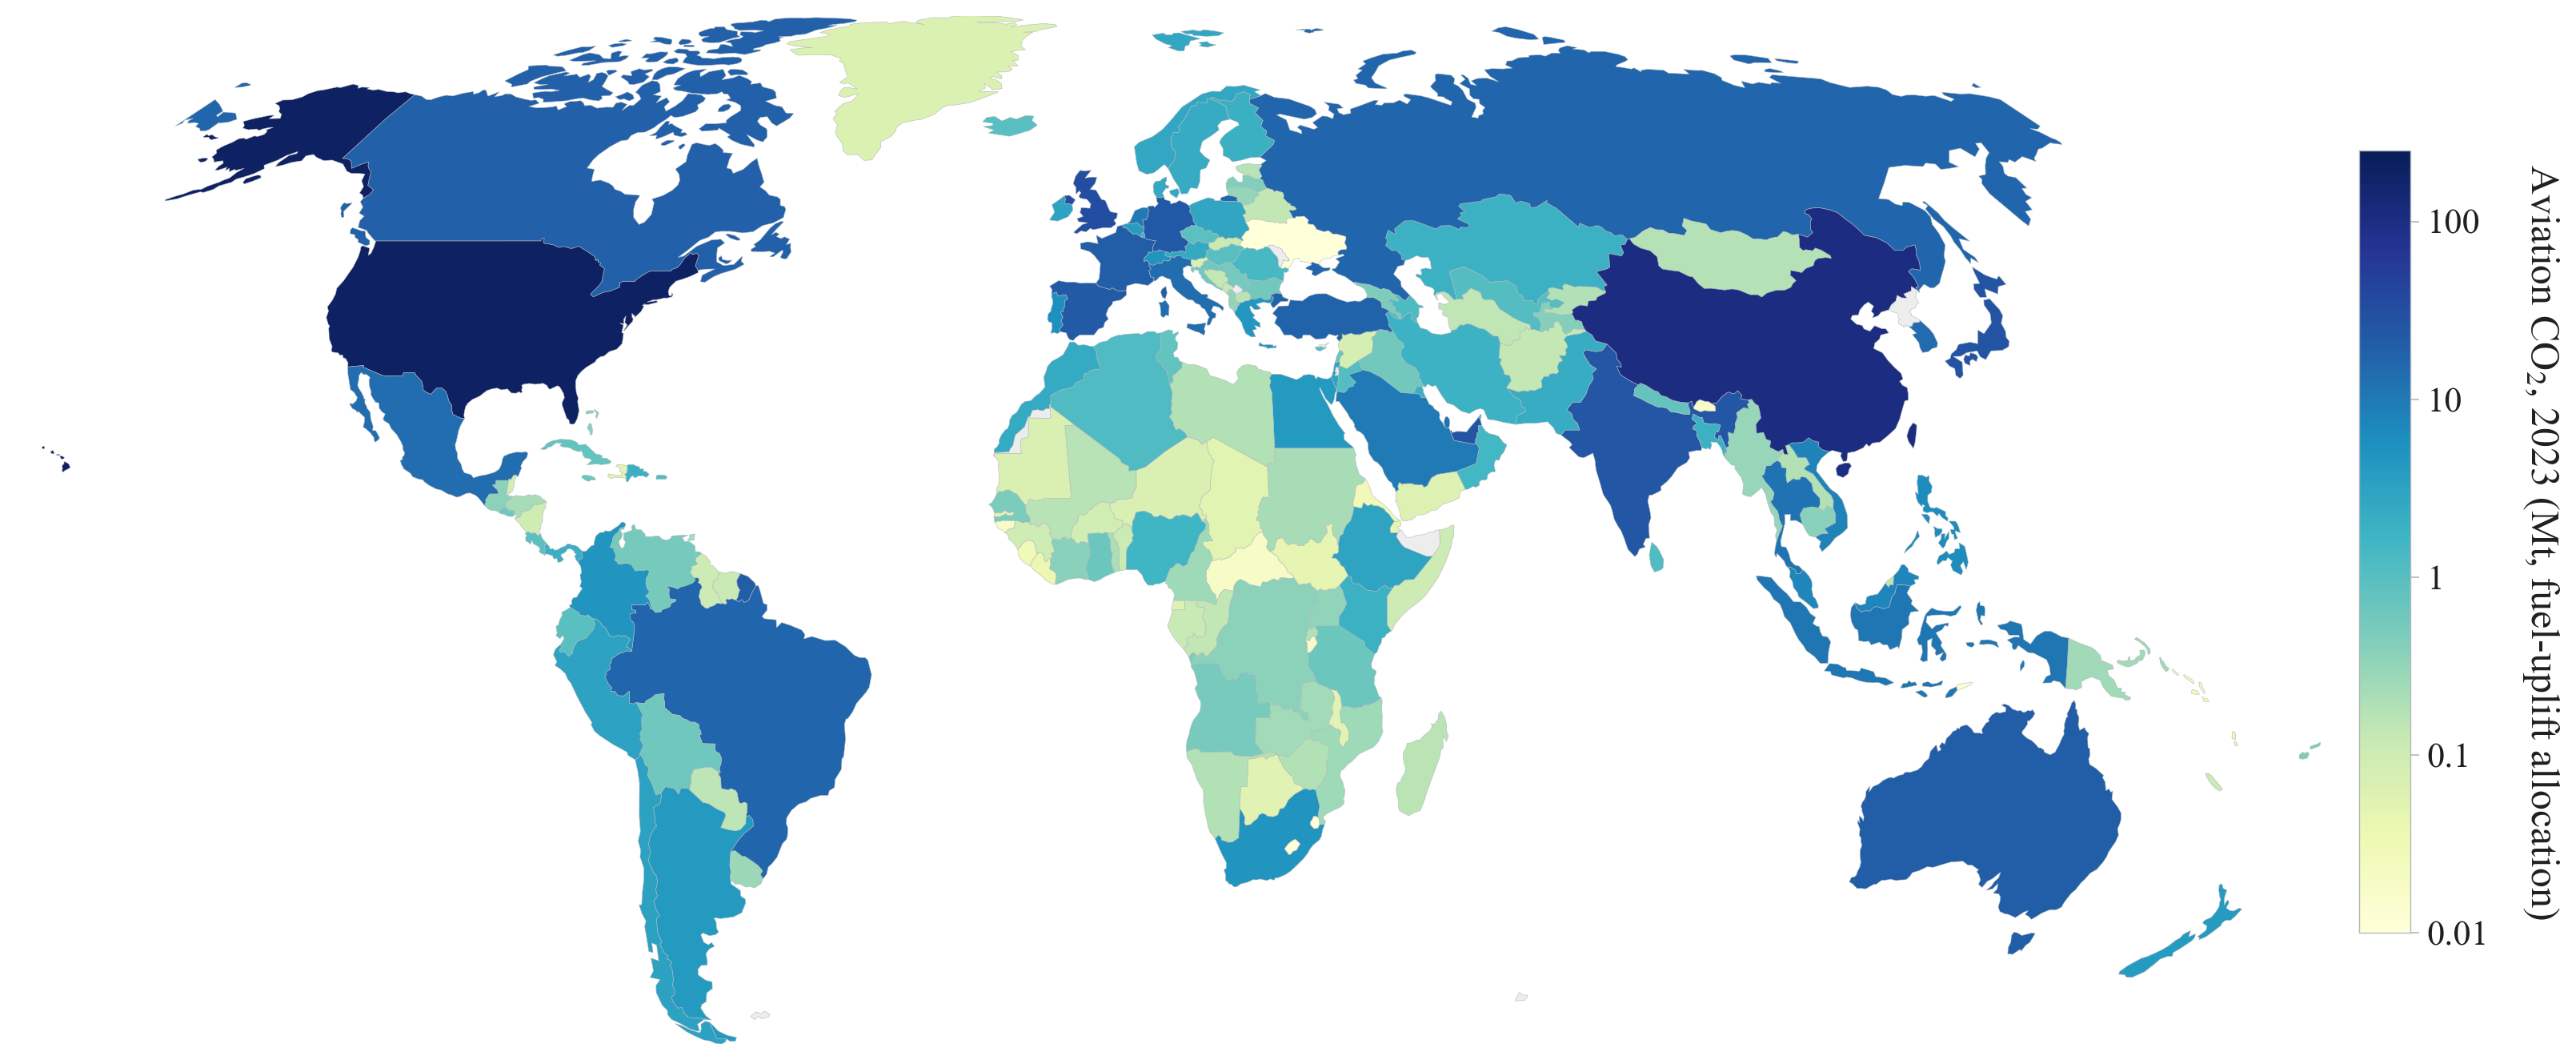
\includegraphics[width=0.92\textwidth]{CO2_map_levels_2023.png}
\caption{Aviation CO$_2$ levels under the bunker convention, 2023.}
\label{fig:levels}
\end{figure}

\begin{figure}[htbp]
\centering
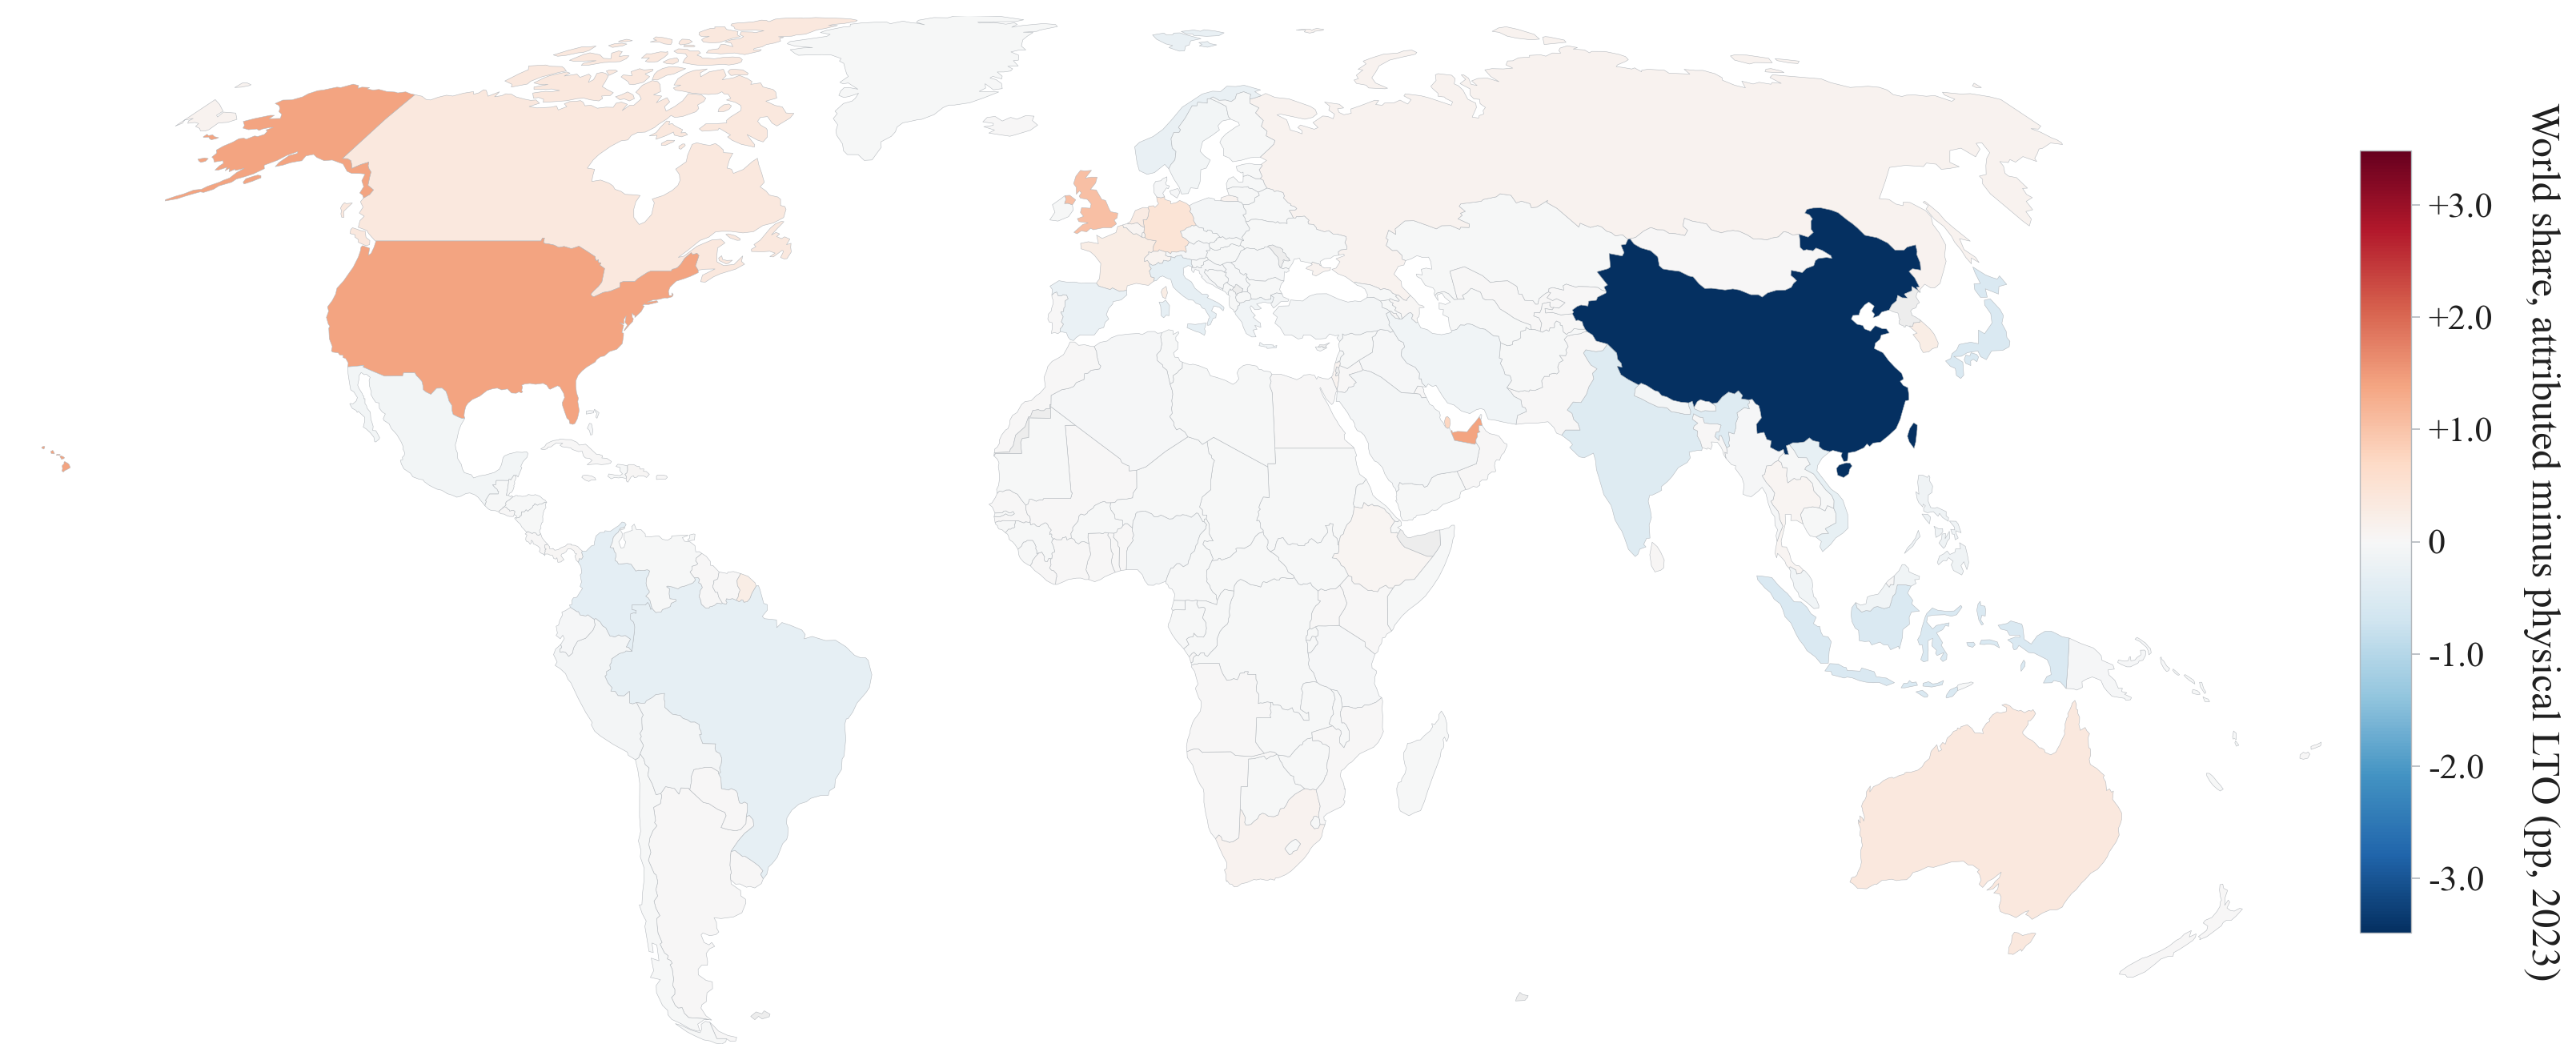
\includegraphics[width=0.92\textwidth]{CO2_map_mismatch_2023.png}
\caption{Attribution mismatch, 2023: bunker-attributed share minus physical LTO share (percentage points). Positive values indicate international hub countries; negative values indicate domestically oriented networks.}
\label{fig:mismatch}
\end{figure}

%=======================================================================
\section{Discussion}
%=======================================================================
Three implications follow from the results. First, for climate policy, the
efficiency gains that accompany network development are not a
decarbonisation strategy. The technique margin is present at both the
country and airport levels, but it offsets less than one tenth of the scale
response, and the scenario calculations indicate that only sustained fuel
switching materially lowers the emissions level. Policies that promote
connectivity on economic grounds should therefore be evaluated jointly with
fuel and demand-side instruments rather than on the expectation that hub
efficiency will absorb the growth in traffic.

Second, for the geography of mitigation burden, the results identify two
distinct wedges. The spillover estimates show that a country's emissions
respond to its neighbours' connectivity, so national accounting misses a
regional externality: a country's traffic shifts toward larger-gauge,
international service as nearby hubs grow, even without growth in its own
connectivity. The attribution analysis shows in addition that accounting
conventions reallocate measured responsibility across countries by up to
3.5 percentage points of the world total. Both wedges bear directly on the
design of instruments, such as CORSIA, that assign obligations on the basis
of booked emissions.

Third, several limitations qualify the estimates. Emissions are
schedule-based and do not reflect load factors, so they measure the carbon
content of scheduled capacity. The primary instrument is strongest in the
network-expansion era, and the later-period elasticity is identified only
when the COVID-19 collapse years are excluded. No causal estimate is
available at the airport level. The
attribution and fuel-switching calculations are partial-equilibrium
accounting exercises, and non-CO$_2$ climate effects of aviation are
outside the scope of the paper. Two extensions are in progress: an
accident-exposure instrument at the airline-year and airport-year level
[YIFU], and base-year bilateral route shares that would permit tracing
spillovers and attribution along individual network links [FANGYU].

%=======================================================================
\appendix
\section{Instrument validity}
%=======================================================================
This appendix reports the evidence behind the identification claims in
Section 4.

\paragraph{Size-by-cycle stress test.} A mechanical concern with any
shifter of the form (global cycle $\times$ baseline characteristic) is that
it may proxy (global cycle $\times$ country size) rather than the intended
geography. We therefore re-estimate each first stage adding interactions of
the global cycle with baseline population, GDP, and airport capacity. The
Feyrer instrument survives: the first-stage $F$ declines only from 120.1 to
115.5 (population and GDP) to 105.8 (adding capacity). The tourism
instrument does not (13.8 to 4.8/4.1 to 0.0--0.6), which is why it is used
only as a lens on the composition margin. An airport-level
heritage-proximity pilot fails the same test (59.5 to 2.3) and was
abandoned; airport-level results in the paper are accordingly descriptive.

\paragraph{Plausibly exogenous bounds.} Following the Conley et al.\
plausibly-exogenous approach, we compute union confidence intervals
allowing the instrument a direct effect $\gamma$ of up to a given share of
the reduced form. For international CO$_2$, the breakdown share is
$f^{*} = 0.85$, and the interval at a 30 percent share is $[3.25, 4.67]$;
for total CO$_2$ the breakdown share is likewise 0.85, and for intensity
0.42. A direct effect amounting to most of the reduced form would be
required to overturn the qualitative conclusions.

\paragraph{Quintile reduced forms.} Figure~\ref{fig:rfquintile} reports
reduced-form slopes by baseline quintile under the tourism shifter, which
are concentrated in low-income, low-connectivity quintiles, consistent with
the split-sample gradient in Table~\ref{tab:hetero}.

% [TODO: overidentification combining feyrer_int and tourism_int with the
%  LATE-difference discussion.]

\begin{figure}[htbp]
\centering
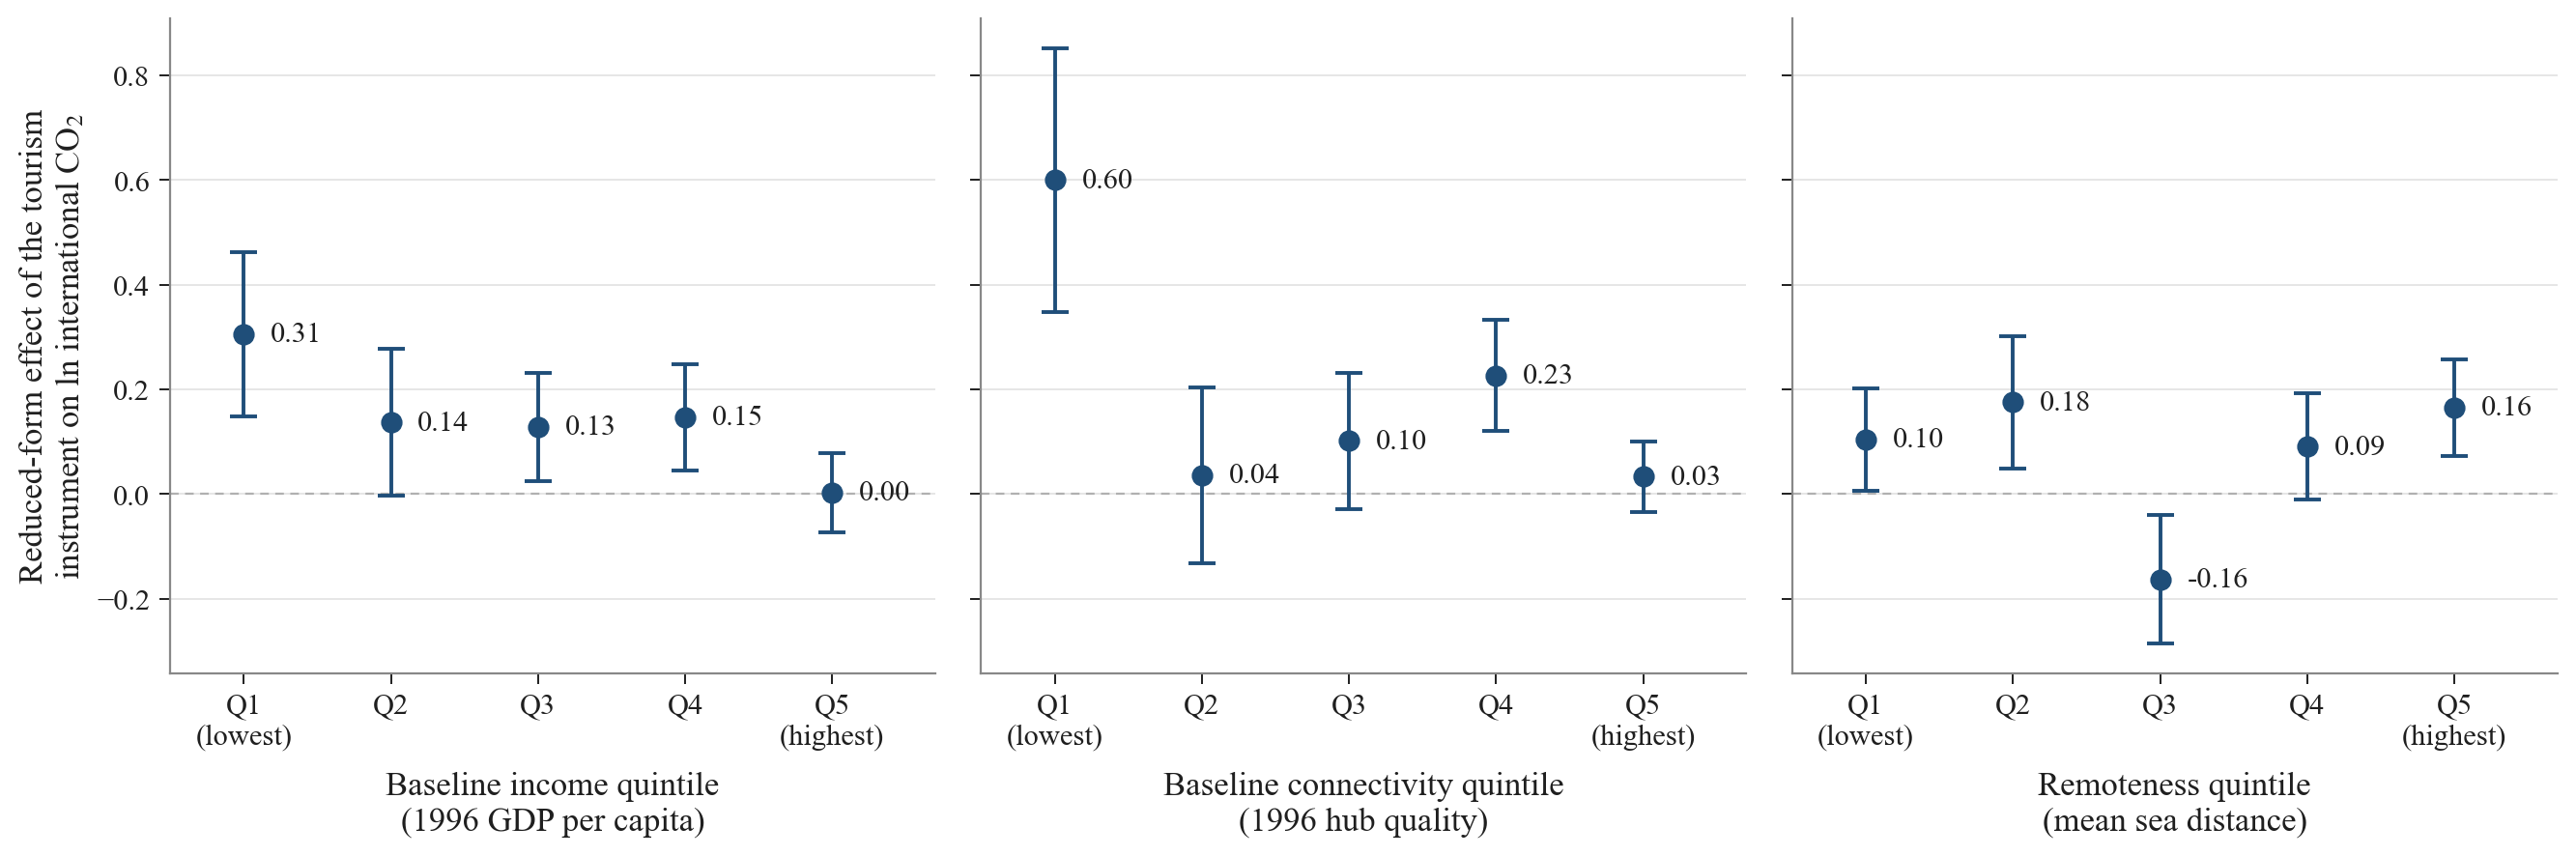
\includegraphics[width=0.92\textwidth]{CO2_rf_quintile.png}
\caption{Reduced-form quintile slopes under the tourism shifter: effects are concentrated in low-income, low-connectivity quintiles.}
\label{fig:rfquintile}
\end{figure}

% Carbon-intensity-of-trade-gains map retained from the heritage pipeline
% (v1 framing, dropped from the main text per Sunbin; kept as appendix
% material pending a decision).
\begin{figure}[htbp]
\centering
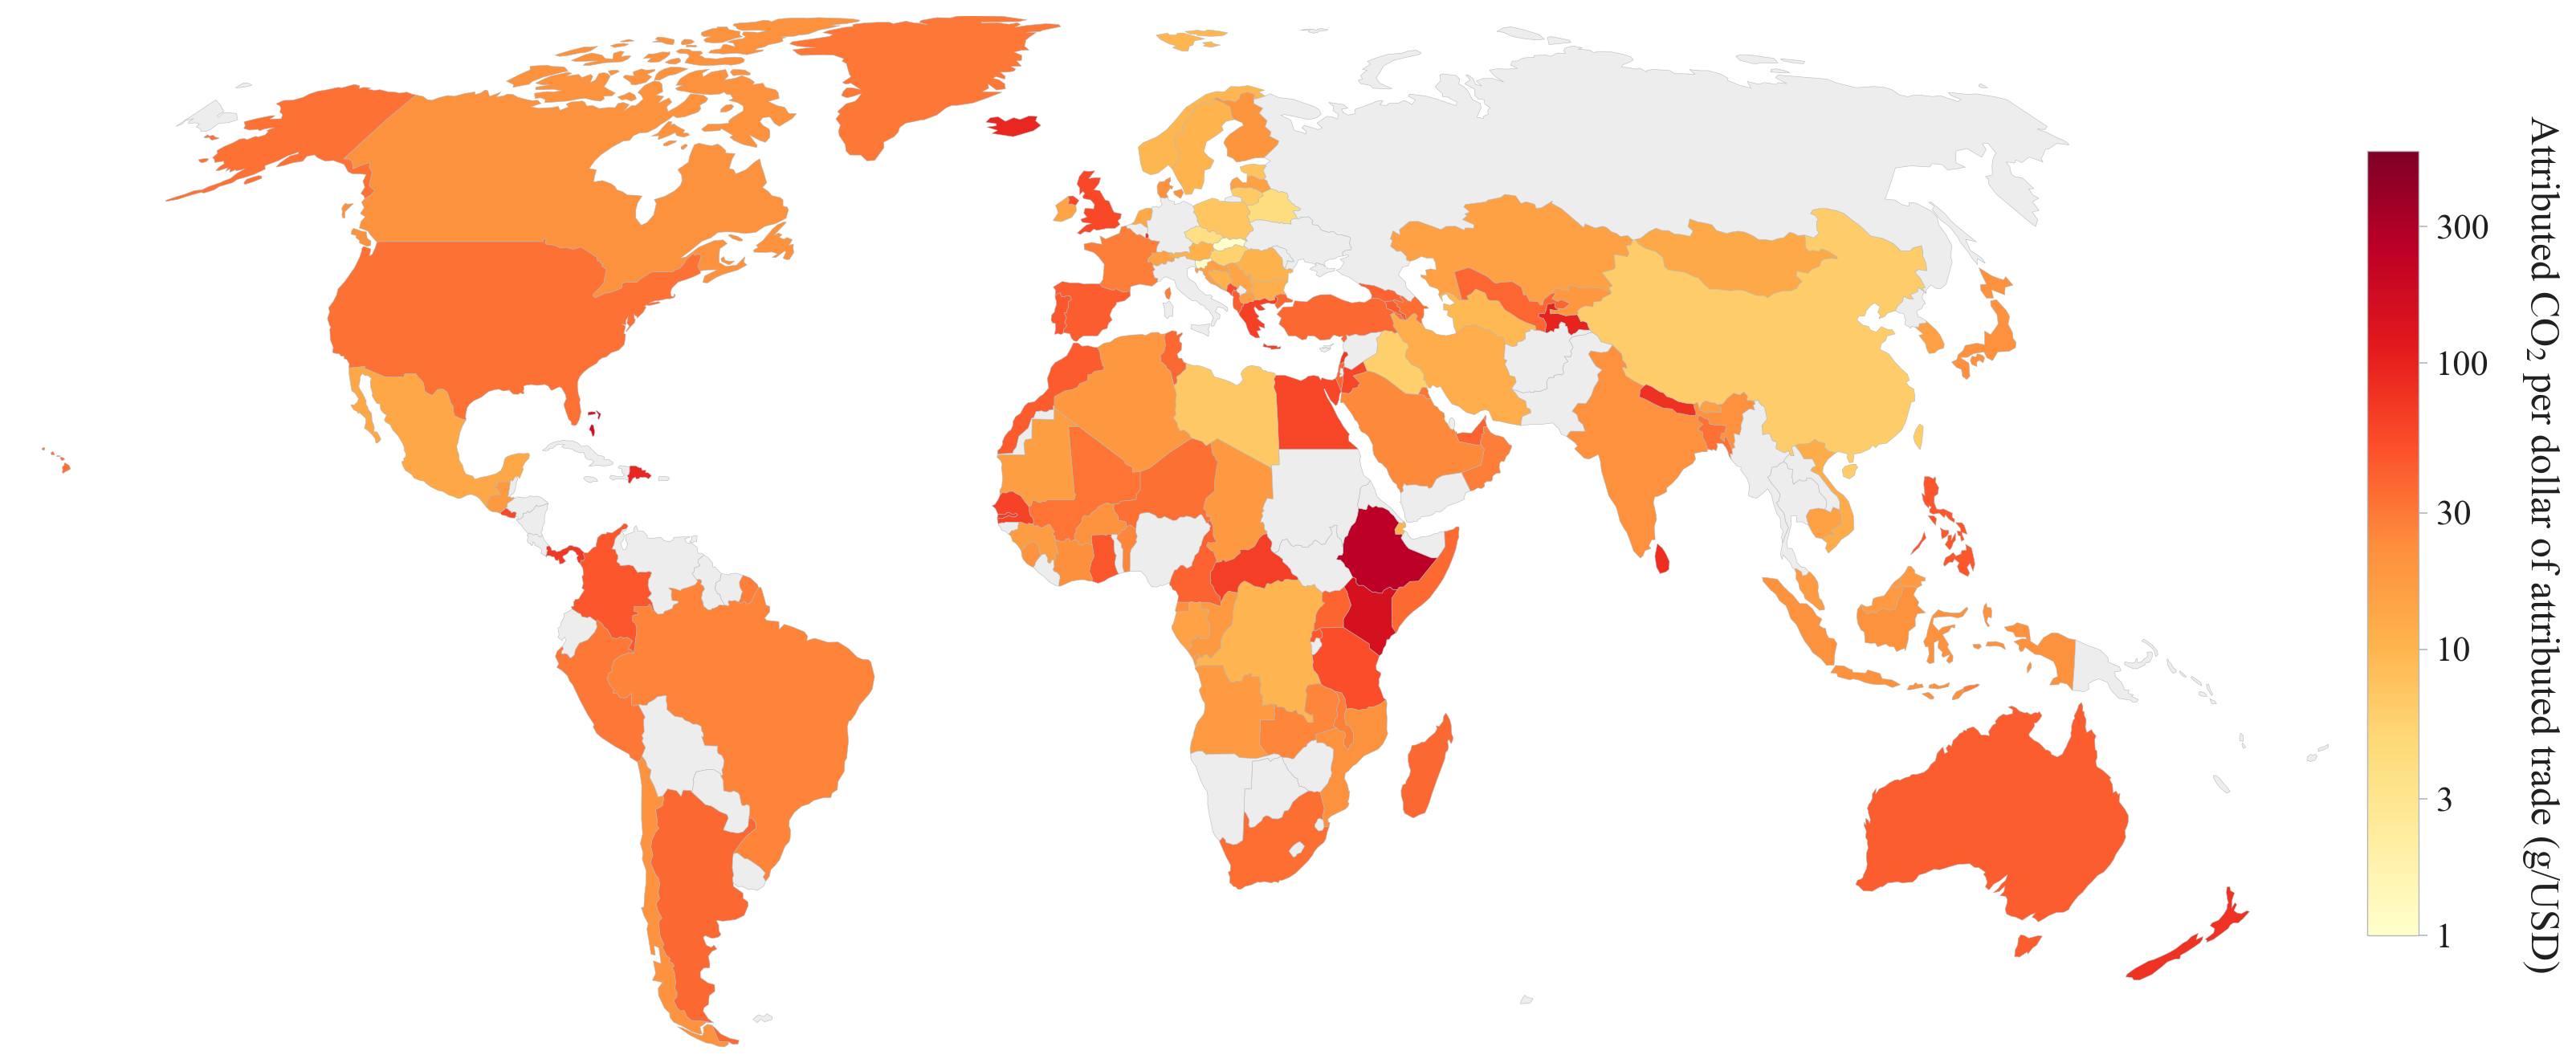
\includegraphics[width=0.92\textwidth]{CO2_map_carbonprice.png}
\caption{Carbon intensity of connectivity gains (g CO$_2$ per USD of trade gain; heritage-instrument pipeline).}
\label{fig:carbonprice}
\end{figure}

\end{document}
